\documentclass[11pt]{article}

\usepackage[T1]{fontenc}
\usepackage[utf8]{inputenc}
\usepackage{lmodern}
\usepackage{microtype}
\usepackage[margin=0.92in]{geometry}
\usepackage{amsmath,amssymb,amsthm,mathtools,bm}
\usepackage{booktabs,longtable,array,tabularx,multirow}
\usepackage{graphicx}
\usepackage{xcolor}
\usepackage{enumitem}
\usepackage{fancyhdr}
\usepackage{hyperref}
\usepackage[nameinlink,noabbrev]{cleveref}
\usepackage{float}
\usepackage{caption}
\usepackage{listings}
\usepackage{url}

\definecolor{navy}{RGB}{24,55,95}
\definecolor{teal}{RGB}{20,105,108}
\definecolor{gold}{RGB}{158,110,22}
\definecolor{softblue}{RGB}{237,244,250}
\definecolor{softgold}{RGB}{252,247,233}
\definecolor{softgray}{RGB}{246,246,246}
\definecolor{darkgreen}{RGB}{25,100,62}
\definecolor{darkred}{RGB}{145,42,42}

\hypersetup{
  colorlinks=true,
  linkcolor=navy,
  citecolor=darkgreen,
  urlcolor=teal,
  pdftitle={Dyadic Radon Profiles in the Fabius--Rvachev Web},
  pdfauthor={Research report for Vladimir Reshetnikov}
}

\pagestyle{fancy}
\fancyhf{}
\fancyhead[L]{\small Dyadic Radon profiles}
\fancyhead[R]{\small \thepage}
\setlength{\headheight}{14pt}

\numberwithin{equation}{section}
\setcounter{tocdepth}{2}
\setcounter{secnumdepth}{3}

% Canonical project-wide mathematical notation.
% Canonical mathematical notation for active FabiusFunction LaTeX documents.
%
% This file is intentionally a plain TeX input rather than a LaTeX package.
% Every standalone document loads it by an explicit path relative to that
% document's directory; included fragments inherit the definitions from their
% root document.  Keep this file independent of document layout and metadata.
%
% Contract:
%   * one command has one mathematical meaning throughout the active corpus;
%   * names encode semantic roles rather than a document-local choice of letter;
%   * visually similar but differently normalized objects have different print;
%   * every command below is defined normatively in the notation catalogue.
%
% The active corpus excludes docs/archive/.  Historical sources may retain
% their original notation only inside an explicitly labelled quotation.

\makeatletter
\@ifundefined{mathbb}{%
  \PackageError{fabius-notation}{The amssymb package must be loaded first}%
    {Load amsmath and amssymb before inputting fabius-notation.tex.}%
}{}
\@ifundefined{operatorname}{%
  \PackageError{fabius-notation}{The amsmath package must be loaded first}%
    {Load amsmath before inputting fabius-notation.tex.}%
}{}
\makeatother

% Version stamp used by the catalogue and by static audits.
\newcommand{\FabiusNotationVersion}{2026-08-31}

% Number systems.  NaturalNumbers is explicitly the nonnegative convention.
\newcommand{\NaturalNumbers}{\mathbb{N}_{0}}
\newcommand{\PositiveIntegers}{\mathbb{N}_{>0}}
\newcommand{\IntegerNumbers}{\mathbb{Z}}
\newcommand{\RationalNumbers}{\mathbb{Q}}
\newcommand{\RealNumbers}{\mathbb{R}}
\newcommand{\ComplexNumbers}{\mathbb{C}}
\newcommand{\ExtendedRealNumbers}{\overline{\mathbb{R}}}

% The three principal Fabius--Rvachev functions.  Subscripts are deliberate:
% a bare F and a calligraphic F have several unrelated uses in the corpus.
\newcommand{\FabiusBounded}{F_{\mathrm{bd}}}
\newcommand{\FabiusGlobal}{F_{\mathrm{gl}}}
\newcommand{\FabiusQuantile}{Q_{F}}
\newcommand{\FabiusClampedQuantile}{Q_{F,\mathrm{cl}}}
\newcommand{\RvachevUp}{\operatorname{up}}

% Constants, elementary operators, and delimiters.
\newcommand{\EulerE}{\mathrm{e}}
\newcommand{\ImaginaryUnit}{\mathrm{i}}
\newcommand{\Differential}{\mathop{}\!\mathrm{d}}
\newcommand{\AbsoluteValue}[1]{\left\lvert #1\right\rvert}
\newcommand{\Norm}[1]{\left\lVert #1\right\rVert}
\newcommand{\Floor}[1]{\left\lfloor #1\right\rfloor}
\newcommand{\Ceiling}[1]{\left\lceil #1\right\rceil}
\newcommand{\FractionalPart}[1]{\left\{#1\right\}}
\newcommand{\PositivePart}[1]{\left(#1\right)_{+}}
\newcommand{\IndicatorOf}[1]{\mathbf{1}_{#1}}
\newcommand{\SetOf}[1]{\left\{#1\right\}}
\newcommand{\InnerProduct}[1]{\left\langle #1\right\rangle}
\newcommand{\CardinalityOf}[1]{\left\lvert #1\right\rvert}
\newcommand{\DefinitionEquals}{\mathrel{\coloneqq}}
\newcommand{\Sign}{\operatorname{sgn}}
\newcommand{\IdentityOperator}{\operatorname{id}}
\newcommand{\SpanOperator}{\operatorname{span}}
\newcommand{\TraceOperator}{\operatorname{tr}}
\newcommand{\RankOperator}{\operatorname{rank}}
\newcommand{\DiagonalOperator}{\operatorname{diag}}
\newcommand{\ResidueOperator}{\operatorname*{Res}}
\newcommand{\LeastCommonMultiple}{\operatorname{lcm}}
\newcommand{\OrderOperator}{\operatorname{ord}}
\newcommand{\PrincipalLogarithm}{\operatorname{Log}}
\newcommand{\FallingFactorial}[2]{\left(#1\right)^{\underline{#2}}}
\newcommand{\RisingFactorial}[2]{\left(#1\right)^{\overline{#2}}}

% Support, topology, convolution, and metric notation.
\newcommand{\SupportOperator}{\operatorname{supp}}
\newcommand{\SupportOf}[1]{\SupportOperator\!\left(#1\right)}
\newcommand{\TopologicalSupportOf}[1]{\operatorname{tsupp}\!\left(#1\right)}
\newcommand{\Convolution}{\mathbin{*}}
\newcommand{\MetricDistance}{\operatorname{dist}}
\newcommand{\TotalVariationDistance}{d_{\mathrm{TV}}}

% Probability.  Equality and convergence in law are not metric distance.
\newcommand{\Probability}{\mathbb{P}}
\newcommand{\Expectation}{\mathbb{E}}
\newcommand{\Variance}{\operatorname{Var}}
\newcommand{\Covariance}{\operatorname{Cov}}
\newcommand{\LawOperator}{\operatorname{Law}}
\newcommand{\LawOf}[1]{\LawOperator\!\left(#1\right)}
\newcommand{\EqualInLaw}{\mathrel{\overset{\mathrm{law}}{=}}}
\newcommand{\ConvergesInLaw}{\mathrel{\xrightarrow{\mathrm{law}}}}

% Fourier and integral transforms.  The printed labels expose normalization.
% FourierTwoPi uses exp(-2*pi*i*x*xi); FourierAngular uses exp(-i*x*omega).
\newcommand{\FourierTwoPi}[1]{\widehat{#1}_{\,2\pi}}
\newcommand{\FourierAngular}[1]{\widehat{#1}_{\,\mathrm{ang}}}
\newcommand{\LaplaceTransformSymbol}{\mathcal{L}}
\newcommand{\MellinTransformSymbol}{\mathcal{M}}
\newcommand{\LaplaceTransformOf}[1]{\LaplaceTransformSymbol\!\left[#1\right]}
\newcommand{\MellinTransformOf}[1]{\MellinTransformSymbol\!\left[#1\right]}
\newcommand{\MomentGeneratingFunction}[1]{M_{#1}}
\newcommand{\CharacteristicFunction}[1]{\varphi_{#1}}

% The two standard sinc functions must never share one symbol.
\newcommand{\SincRad}{\operatorname{sinc}_{\mathrm{rad}}}
\newcommand{\SincPi}{\operatorname{sinc}_{\pi}}

% Binary arithmetic and Thue--Morse notation.
\newcommand{\BinaryDigitSum}{\operatorname{wt}_{2}}
\newcommand{\ThueMorseSignSymbol}{\varepsilon}
\newcommand{\ThueMorseSign}[1]{\varepsilon_{#1}}
\newcommand{\PadicValuation}[1]{\nu_{#1}}
\newcommand{\TwoAdicValuation}{\nu_{2}}

% q-series notation.  Every base is an explicit argument.
\newcommand{\QPochhammer}[3]{\left(#1;#2\right)_{#3}}
\newcommand{\GaussianBinomial}[3]{%
  \genfrac{[}{]}{0pt}{}{#1}{#2}_{#3}%
}
\newcommand{\QInteger}[2]{\left[#1\right]_{#2}}

% Named special functions.
\newcommand{\Polylogarithm}{\operatorname{Li}}
\newcommand{\LambertW}{W}
\newcommand{\GammaFunction}{\Gamma}
\newcommand{\RiemannZeta}{\zeta}

% Asymptotics.  BigO and LittleO are operator tokens for existing formula
% grammar; prefer the At forms so that the limiting regime is printed.
\newcommand{\BigO}{\mathcal{O}}
\newcommand{\LittleO}{o}
\newcommand{\BigOAt}[2]{\mathcal{O}_{#2}\!\left(#1\right)}
\newcommand{\LittleOAt}[2]{o_{#2}\!\left(#1\right)}

\newtheorem{theorem}{Theorem}[section]
\newtheorem{proposition}[theorem]{Proposition}
\newtheorem{lemma}[theorem]{Lemma}
\newtheorem{corollary}[theorem]{Corollary}
\newtheorem{conjecture}[theorem]{Conjecture}
\newtheorem{problem}[theorem]{Problem}
\theoremstyle{definition}
\newtheorem{definition}[theorem]{Definition}
\newtheorem{example}[theorem]{Example}
\newtheorem{algorithm}[theorem]{Algorithm}
\theoremstyle{remark}
\newtheorem{remark}[theorem]{Remark}
\newtheorem{caution}[theorem]{Caution}

\newcommand{\Bell}{\mathcal B}
\newcommand{\New}{\textcolor{darkgreen}{\textsf{\textbf{[N]}}}}
\newcommand{\Imported}{\textcolor{navy}{\textsf{\textbf{[I]}}}}
\newcommand{\Evidence}{\textcolor{gold}{\textsf{\textbf{[E]}}}}
\newcommand{\Conj}{\textcolor{darkred}{\textsf{\textbf{[C]}}}}

\newenvironment{resultbox}[1]{%
  \begin{center}\begin{minipage}{0.94\textwidth}
  \color{navy}\hrule\vspace{0.55em}
  \textbf{#1}\par\smallskip\color{black}
}{%
  \vspace{0.55em}\color{navy}\hrule
  \end{minipage}\end{center}
}

\lstdefinestyle{frontiercode}{
  language=Python,
  basicstyle=\ttfamily\footnotesize,
  backgroundcolor=\color{softgray},
  frame=single,
  rulecolor=\color{gray},
  breaklines=true,
  columns=fullflexible,
  showstringspaces=false,
  keywordstyle=\color{navy}\bfseries,
  commentstyle=\color{teal},
  stringstyle=\color{gold!80!black},
  xleftmargin=0.6em,xrightmargin=0.6em
}

\begin{document}
\hypersetup{pageanchor=false}
\begin{titlepage}
\centering
\vspace*{1.1cm}
{\color{navy}\rule{0.84\textwidth}{1.2pt}}\\[0.95cm]
{\Huge\bfseries\color{navy} Dyadic Radon Profiles in the\\[0.16em] Fabius--Rvachev Web\par}
\vspace{0.65cm}
{\Large\color{teal} Spectral reconstruction, generalized Thue--Morse signs,\\
$q$-sampled cumulants, Pascal factorizations, and Lambert frontiers\par}
\vspace{0.95cm}
{\color{navy}\rule{0.84\textwidth}{0.6pt}}\\[1.15cm]
{\large A corpus-audited frontier research report\par}
\vspace{0.25cm}
{\large prepared for Vladimir Reshetnikov\par}
\vfill
{\large 30 August 2026\par}
\vspace{0.55cm}
{\small Based on a recursive review of the current and historically indexed
\texttt{*.tex} corpus under\\[0.25em]
\url{https://github.com/VladimirReshetnikov/ProveIt/tree/main/Analysis/FabiusFunction/docs}\par}
\end{titlepage}
\hypersetup{pageanchor=true}
\pagenumbering{roman}

\begin{abstract}
The Fabius--Rvachev documentation corpus already contains a large network of
results on the signed Thue--Morse sequence, exact dyadic Fabius values,
$q$-Pochhammer and Gaussian-binomial formulae, infinite sinc products,
Bernoulli and Bell cumulants, Legendre representations, inverse-Fabius
Lambert--$W$ asymptotics, and several higher-rank spectral constructions.  The
present report begins at a boundary not found in the audited sources: a
\emph{tomographic classification} of all dyadic linear projections built from
independent copies of the classical Rvachev law.

For a nonnegative integer direction profile $c=(c_h)_{h\ge0}$ satisfying
$\sum_hc_h2^{-h}<\infty$, let
\[
 Y_c=\sum_{h\ge0}\sum_{\ell=1}^{c_h}2^{-h}X_{h,\ell},
\]
where the $X_{h,\ell}$ are independent centered Rvachev variables.  Its
Fourier transform is
\[
 \Psi_c(t)=\prod_{j\ge0}\SincPi(t/2^j)^{a_j},
 \qquad a_j=\sum_{h\le j}c_h,
\]
and the zero at any integer of $2$-adic valuation $v$ has multiplicity
\[
 m_v=\sum_{h=0}^{v}c_h(v-h+1).
\]
The first principal theorem proves that this spectral profile determines the
projection uniquely:
\[
 c_v=m_v-2m_{v-1}+m_{v-2}.
\]
Thus dyadic direction profiles are in bijection with nonnegative
integer-valued discretely convex zero-multiplicity sequences.  Their generating
functions satisfy
\[
 A(q)=\frac{C(q)}{1-q},\qquad
 M(q)=\frac{C(q)}{(1-q)^2},\qquad
 \mathcal Z_c(s)=\zeta(s)\frac{C(2^{-s})}{1-2^{-s}}.
\]

A second group of results shows that every normalized even-cumulant ratio is a
$q$-sample of the same direction polynomial or power series:
\[
 \frac{\kappa_{2n}(Y_c)}{\kappa_{2n}(X)}=C(4^{-n}).
\]
The shifted ratio sequence is therefore a Hausdorff moment sequence carried by
the dyadic grid $\{4^{-h}\}$; all alternating finite differences and Hankel
minors are nonnegative.  Bell-polynomial moments and Legendre coefficients
become finite transforms of these $q$-samples.  A third theorem classifies the
spectral sign sequence
\[
 \varepsilon_c(N)=(-1)^{\sum_j(a_j\bmod2)b_j(N)}:
\]
it is $2$-automatic exactly when the parity word $(a_j\bmod2)$ is eventually
periodic, and finite blocks have a precisely computable Prouhet cancellation
order.  A fourth theorem proves the sharp logarithmic Fourier envelope for
regularly growing exponents $a_j\sim A j^d$:
\[
 \limsup_{x\to\infty}\frac{\log|\Psi_c(x)|}{(\log x)^{d+2}}
 =-\frac{A}{(d+1)(d+2)(\log2)^{d+1}}.
\]

The existing Pascal--Rvachev hierarchy receives a new geometric
factorization: its rank-$r$ law is an explicit infinite Radon projection of
classical rank-one Rvachev variables, with scale multiplicities
$\binom{h-1}{r-2}$.  The report also derives exact positive dyadic-comb
cubature for every profile, an inverse-Fabius coordinate representation of the
whole projection cone, and a detailed conjectural Lambert--$W$ endpoint
program.  Fully commented Python code, exact CSV tables, vector and raster
figures, the source-audit ledger, build instructions, and checksums accompany
the manuscript.  The word ``new'' throughout means apparently new relative to
the audited repository corpus, not a claim of worldwide historical priority.
\end{abstract}

\tableofcontents
\clearpage
\pagenumbering{arabic}

\section{Scope, audit method, and contribution boundary}
\label{sec:audit}

\subsection{The living documentation tree}

The requested source is not a single article.  At the inspected snapshot it
contains a primary Fabius--Rvachev exposition, a mathematical glossary, a
non-elementarity paper, a Lean walkthrough, transcribed source papers, a
frozen archive, and a semi-formalized frontier system.  The latter was
reorganized on 28 August 2026 into thematic consolidated volumes.  Therefore
a filename count from an earlier checkout is not, by itself, a reliable map of
current mathematical content.

The audit used three complementary layers.
\begin{enumerate}[label=\textbf{A\arabic*.},leftmargin=*]
\item The current public tree, the current frontier README, the current draft
      manifest, and the principal consolidated sources were inspected at the
      level of theorem statements, proof interfaces, open problems, and result
      registers.
\item A preserved path-complete ledger from 27 August 2026 was used to retain
      coverage of paths later absorbed into consolidated manuscripts.  It
      records 78 visible TeX paths at that checkpoint, including generated
      table fragments; another preserved audit records 57 distinct theorem-
      bearing artifacts under a different deduplication convention.  The
      discrepancy is explained by consolidation, generated fragments, and
      frozen revisions, not by ignored source families.
\item Prior frontier packages in the user's file library were phrase- and
      formula-searched for every candidate structure developed below.
      Rediscovered material was removed from the novelty ledger.
\end{enumerate}
The complete historical path ledger is included in the archive as
\path{corpus_inventory_2026-08-27.txt}; the current claim-oriented audit is
included as \path{CORPUS_AUDIT.md}.

\subsection{Established material treated as input}

The report does \emph{not} relabel the following as new:
\begin{itemize}[leftmargin=*]
\item the random-uniform series for the centered Rvachev law and its compactly
      supported $C^\infty$ density;
\item the Fabius/Rvachev functional-differential equations, exact dyadic
      values, rational moments, and the $q=1/2$ Gaussian-binomial formulae;
\item Bernoulli cumulants, complete Bell-polynomial moments, Appell
      deconvolution, and polynomial synthesis by shifted up-functions;
\item the canonical infinite sinc product, integer zero multiplicities
      $1+\TwoAdicValuation(n)$, arithmetic rays, spectral determinants, and Fourier-decay
      analyses;
\item the Pascal--Rvachev product hierarchy, its existing zero divisor,
      generalized spectral signs, spectral zeta function, endpoint saddle, and
      rank asymptotics;
\item self-sampling and dyadic-comb quadrature in the classical and previously
      developed higher-rank settings;
\item Legendre, Jacobi, Chebyshev, Lagrange, and repeated-integration
      representation schemes;
\item inverse-Fabius algebraic germs, all-orders Lambert--Bell asymptotics,
      quantile transforms, and the existing integration/fractional-calculus
      corpus;
\item cyclotomic $q$-limits, root-of-unity natural boundaries, Stein--Koopman
      calculus, and free/Boolean cumulant investigations developed in prior
      packages.
\end{itemize}
These statements are imported interfaces, marked \Imported.  The new layer is
their composition through a general dyadic direction profile.

\subsection{Result ledger}

\begin{longtable}{@{}p{0.08\textwidth}p{0.34\textwidth}p{0.50\textwidth}@{}}
\caption{Principal results and proof status.}\label{tab:result-ledger}\\
\toprule
ID & Result & Contribution \\
\midrule
\endfirsthead
\toprule ID & Result & Contribution \\
\midrule
\endhead
R1 & \New\ Profile law & Infinite-dimensional Radon projection, support, smooth density, and cumulative sinc exponents.\\
R2 & \New\ Spectral inversion & Exact formula $c_v=\Delta^2m_v$ and classification by discrete convexity.\\
R3 & \New\ Zero-zeta transform & $\mathcal Z_c(s)=\zeta(s)C(2^{-s})/(1-2^{-s})$.\\
R4 & \New\ Cumulant $q$-sampling & $\kappa_{2n}(Y_c)/\kappa_{2n}(X)=C(4^{-n})$.\\
R5 & \New\ Hausdorff rigidity & Complete monotonicity, Hankel positivity, and uniqueness of the direction profile from cumulants.\\
R6 & \New\ Digital sign classification & Automaticity iff the exponent-parity word is eventually periodic; exact Prouhet order.\\
R7 & \New\ Sharp Fourier envelope & Exact limsup constant for $a_j\sim Aj^d$.\\
R8 & \New\ Pascal factorization & Every Pascal rank is an explicit dyadic projection of classical up-laws.\\
R9 & \New\ Profile cubature & Sharp uniform degree for positive dyadic-comb rules from $m_H$.\\
R10 & \New\ Inverse-Fabius coordinates & Exact representation of all profile laws by independent inverse-Fabius variables.\\
R11 & \Evidence\ Computation & Exact finite-difference, Prouhet, Hankel, zeta, and high-precision envelope tests.\\
R12 & \Conj\ Frontier program & Spectral rigidity, Lambert transseries, tomography, stability, and matrix-dilation extensions.\\
\bottomrule
\end{longtable}

\begin{resultbox}{Proof-status convention}
A theorem labelled \New\ is proved in this report.  A statement labelled
\Imported\ is taken from the audited Fabius--Rvachev corpus or from a standard
classical source and is restated only to fix normalization.  Numerical claims
are labelled \Evidence; conjectures and research problems are labelled
\Conj.  Computation is never used as a substitute for a proof.
\end{resultbox}

\section{Normalization and imported rank-one structure}
\label{sec:normalization}

\subsection{The centered Rvachev random variable}

Define the normalized sinc function
\begin{equation}
 \SincPi z:=\frac{\sin(\pi z)}{\pi z},\qquad \SincPi0=1.
 \label{eq:sinc-normalized}
\end{equation}
Let $U_0,U_1,\ldots$ be independent random variables uniformly distributed on
$[-1/2,1/2]$, and put
\begin{equation}
 X:=\sum_{j=0}^{\infty}2^{-j}U_j.
 \label{eq:rank-one-series}
\end{equation}
The series converges absolutely and $|X|\le1$.  We use $\RvachevUp$ for its density.
This is the centered Rvachev up-law in the normalization of the repository.
Its characteristic function in the $2\pi$ Fourier convention is
\begin{equation}
 \Phi(t):=\Expectation\EulerE^{2\pi\ImaginaryUnit tX}
 =\prod_{j=0}^{\infty}\SincPi(t/2^j).
 \label{eq:rank-one-Phi}
\end{equation}
The density is even, nonnegative, $C^\infty$, supported on $[-1,1]$, and flat
at both endpoints.

\subsection{Fabius and inverse-Fabius coordinates}

Let $\FabiusBounded:[0,1]\to[0,1]$ be the standard Fabius function, with
$\FabiusQuantile=\FabiusBounded^{-1}$.  With
\begin{equation}
 G(x):=\Probability(X\le x),\qquad -1\le x\le1,
\end{equation}
we have the exact coordinate relation
\begin{equation}
 G(x)=\FabiusBounded\!\left(\frac{x+1}{2}\right).
 \label{eq:CDF-Fabius}
\end{equation}
Indeed, differentiating the right-hand side and using the two halves of the
Fabius dilation equation gives $G'(x)=\RvachevUp(x)$, while both sides vanish at
$x=-1$.

\begin{proposition}[\Imported\ Inverse-Fabius quantile coordinate]
\label{prop:quantile-coordinate}
If $V\sim\operatorname{Unif}[0,1]$, then
\begin{equation}
 X\ \stackrel d=\ 2\FabiusQuantile(V)-1.
 \label{eq:X-quantile}
\end{equation}
\end{proposition}

\begin{proof}
The quantile of $G(x)=\FabiusBounded((x+1)/2)$ is
$G^{-1}(v)=2\FabiusQuantile(v)-1$.
\end{proof}

\subsection{Bernoulli cumulants}

The moment generating function is
\begin{equation}
 M_X(z)=\Expectation\EulerE^{zX}
 =\prod_{j=0}^{\infty}
   \frac{\sinh(z/2^{j+1})}{z/2^{j+1}}.
 \label{eq:rank-one-mgf}
\end{equation}
Writing $\kappa_n(X)$ for the ordinary cumulants, the repository's
Bernoulli--Mersenne formula is
\begin{equation}
 \kappa_{2n}(X)
 =\frac{2^{2n-1}B_{2n}}{n(4^n-1)},
 \qquad
 \kappa_{2n+1}(X)=0.
 \label{eq:base-cumulants}
\end{equation}
For example,
\begin{equation}
 \kappa_2(X)=\frac19,
 \qquad
 \kappa_4(X)=-\frac{2}{225},
 \qquad
 \kappa_6(X)=\frac{16}{11907}.
\end{equation}
These imported cumulants will serve as spectral probes of the new direction
profiles.

\section{Dyadic Radon profiles}
\label{sec:profiles}

\subsection{Definition and geometric meaning}

\begin{definition}[Dyadic direction profile]
A \emph{dyadic direction profile} is a sequence
$c=(c_h)_{h\ge0}$ of nonnegative integers such that
\begin{equation}
 S_c:=\sum_{h=0}^{\infty}c_h2^{-h}<\infty.
 \label{eq:support-budget}
\end{equation}
For independent copies $X_{h,\ell}$ of $X$, define
\begin{equation}
 Y_c:=\sum_{h=0}^{\infty}\sum_{\ell=1}^{c_h}2^{-h}X_{h,\ell}.
 \label{eq:Yc}
\end{equation}
\end{definition}

The deterministic bound in \eqref{eq:support-budget} makes
\eqref{eq:Yc} absolutely convergent for every point in the underlying product
space.  If only finitely many $c_h$ are nonzero, the law is the ordinary Radon
projection of the product density
$\prod_{h,\ell}\RvachevUp(x_{h,\ell})$ along the coefficient vector whose entries are
$2^{-h}$.  For infinitely many occupied shells it is the compatible
projective limit of those finite-dimensional Radon projections.  This is the
reason for the terminology.

Define the profile generating function and its cumulative exponents by
\begin{equation}
 C(q):=\sum_{h\ge0}c_hq^h,
 \qquad
 a_j:=\sum_{h=0}^{j}c_h,
 \qquad
 A(q):=\sum_{j\ge0}a_jq^j.
 \label{eq:C-A-def}
\end{equation}
The support condition implies convergence of $C(q)$ at least for $|q|<1/2$.
All identities below are also valid formally.

\begin{theorem}[\New\ Radon-profile law]
\label{thm:profile-law}
Let $c$ be a dyadic direction profile.  Then:
\begin{enumerate}[label=\textup{(\roman*)},leftmargin=*]
\item $Y_c$ has support exactly $[-S_c,S_c]$.
\item If $c\ne0$, its law has a nonnegative $C^\infty$ density $g_c$ with
      compact support.
\item Its characteristic function is
\begin{equation}
 \Psi_c(t):=\Expectation\EulerE^{2\pi\ImaginaryUnit tY_c}
 =\prod_{h\ge0}\Phi(t/2^h)^{c_h}
 =\prod_{j\ge0}\SincPi(t/2^j)^{a_j}.
 \label{eq:Psi-profile}
\end{equation}
\item The generating functions satisfy the first triangular integration law
\begin{equation}
 A(q)=\frac{C(q)}{1-q}.
 \label{eq:A-C}
\end{equation}
\end{enumerate}
\end{theorem}

\begin{proof}
The product of intervals
$\prod_{h,\ell}[-1,1]$ is compact, and the linear map
$L_c((x_{h,\ell}))=\sum_{h,\ell}2^{-h}x_{h,\ell}$ is continuous because its
series converges uniformly.  Its image is the Minkowski sum of intervals
$[-2^{-h},2^{-h}]$ repeated $c_h$ times, hence the full interval
$[-S_c,S_c]$.  The product probability measure has full support, so its
push-forward has exactly that support.

Choose the first occupied shell $h_0$ and one of its coordinates.  Write
$Y_c=2^{-h_0}X+R$, with $R$ independent.  The law of $2^{-h_0}X$ has a compactly
supported $C^\infty$ density, and convolving it with the finite measure
$\mathcal L(R)$ preserves $C^\infty$ regularity and nonnegativity.

Independence gives the first product in \eqref{eq:Psi-profile}.  Substitute
\eqref{eq:rank-one-Phi} and collect the factor
$\SincPi(t/2^j)$: it occurs once for every outer shell $h\le j$, with total
multiplicity $a_j$.  Finally,
\[
 A(q)=\sum_{j\ge0}\sum_{h\le j}c_hq^j
 =\sum_{h\ge0}c_h\frac{q^h}{1-q}=\frac{C(q)}{1-q}.
\]
\end{proof}

\begin{proposition}[\New\ Profile addition and renormalization]
\label{prop:profile-monoid}
For profiles $c,d$ and independent variables,
\begin{equation}
 Y_{c+d}\stackrel d=Y_c+Y_d,
 \qquad
 \Psi_{c+d}=\Psi_c\Psi_d.
 \label{eq:profile-addition}
\end{equation}
Let $Tc=(c_{h+1})_{h\ge0}$ be the left shift.  Then
\begin{equation}
 Y_c\stackrel d=
 \sum_{\ell=1}^{c_0}X_\ell+\frac12Y_{Tc}',
 \label{eq:profile-renormalization}
\end{equation}
where all terms on the right are independent, and
\begin{equation}
 C(q)=c_0+qC_{Tc}(q).
\end{equation}
\end{proposition}

\begin{proof}
Both statements are obtained by partitioning the independent coordinates in
\eqref{eq:Yc}.  In the second, reindex $h\mapsto h+1$ in the positive-scale
tail.
\end{proof}

\begin{example}[Classical and polynomial profiles]
The classical up-law is $c=(1,0,0,\ldots)$, so $a_j=1$.  If $c_h=1$ for every
$h$, then $a_j=j+1$, $S_c=2$, and
\[
 \Psi_c(t)=\prod_{j\ge0}\SincPi(t/2^j)^{j+1}.
\]
More generally, choosing
$c_h=(h+1)^d-h^d$ gives $a_j=(j+1)^d$ and produces the full hierarchy of
logarithmic Fourier orders treated in \cref{sec:fourier-envelope}.
\end{example}

\section{Integer zero profiles and exact spectral inversion}
\label{sec:zero-profile}

\subsection{Multiplicity as a second triangular integration}

For $n\in\IntegerNumbers\setminus\{0\}$ write $v=\TwoAdicValuation(|n|)$.  A factor
$\SincPi(t/2^j)$ vanishes at $t=n$ exactly when $j\le v$, and then the zero is
simple.

\begin{theorem}[\New\ Integer-zero profile]
\label{thm:zero-profile}
The zero of $\Psi_c$ at every nonzero integer of $2$-adic valuation $v$ has
multiplicity
\begin{equation}
 m_v:=\OrderOperator_{t=n}\Psi_c(t)
 =\sum_{j=0}^{v}a_j
 =\sum_{h=0}^{v}c_h(v-h+1).
 \label{eq:m-profile}
\end{equation}
If
\begin{equation}
 M(q):=\sum_{v\ge0}m_vq^v,
 \label{eq:M-generating}
\end{equation}
then
\begin{equation}
 M(q)=\frac{A(q)}{1-q}=\frac{C(q)}{(1-q)^2}.
 \label{eq:M-C}
\end{equation}
\end{theorem}

\begin{proof}
The first equality counts the vanishing sinc factors in
\eqref{eq:Psi-profile}.  Substituting $a_j=\sum_{h\le j}c_h$ and reversing the
finite triangular sum gives the second expression.  A second application of
the calculation in \eqref{eq:A-C} gives \eqref{eq:M-C}.
\end{proof}

\subsection{Discrete-convex classification}

Set $m_{-1}=m_{-2}=0$ and use the forward difference
$\Delta m_v=m_v-m_{v-1}$.

\begin{theorem}[\New\ Spectral reconstruction and classification]
\label{thm:classification}
The direction profile is recovered from the integer-zero multiplicities by
\begin{equation}
 \boxed{\ c_v=\Delta^2m_v=m_v-2m_{v-1}+m_{v-2}.\ }
 \label{eq:second-difference-inversion}
\end{equation}
Consequently, a sequence $(m_v)_{v\ge0}$ occurs as the integer-zero profile of
a dyadic Radon projection if and only if
\begin{equation}
 \Delta^2m_v\in\IntegerNumbers_{\ge0}
 \quad\text{for every }v,
 \qquad
 \sum_{v\ge0}(\Delta^2m_v)2^{-v}<\infty.
 \label{eq:classification-conditions}
\end{equation}
The realizing profile is unique.  It has finite support if and only if $m_v$
is eventually affine in $v$.
\end{theorem}

\begin{proof}
From \eqref{eq:m-profile},
\[
 \Delta m_v=a_v,
 \qquad
 \Delta^2m_v=a_v-a_{v-1}=c_v,
\]
with the stated zero initial conditions.  This proves necessity and
uniqueness.  Conversely, if \eqref{eq:classification-conditions} holds, define
$c_v=\Delta^2m_v$.  Twice summing the second differences from the zero initial
conditions reconstructs the original $m_v$ and gives
\eqref{eq:m-profile}; the weighted condition makes $c$ an admissible profile.
Finally, $c_v=0$ eventually exactly when $\Delta^2m_v=0$ eventually, which is
equivalent to eventual affinity.
\end{proof}

\begin{remark}[A monoid isomorphism]
Profile addition corresponds to pointwise addition of zero profiles.  Thus
\cref{thm:classification} identifies the additive cone of dyadic direction
profiles with the additive cone of integer-valued, discretely convex sequences
satisfying the support bound.  The Fourier zero divisor is not merely an
invariant; it is a complete coordinate system for this projection cone.
\end{remark}

\begin{example}[Low-complexity inversions]
\begin{enumerate}[label=\textup{(\alph*)},leftmargin=*]
\item $m_v=v+1$ gives $c_0=1$ and $c_v=0$ for $v\ge1$: the classical law.
\item $m_v=r(v+1)$ gives $c_0=r$ and no other occupied scale: the convolution
      of $r$ independent up-laws.
\item $m_v=\binom{v+2}{2}$ gives $c_v=1$ for all $v$: one coordinate at every
      scale.
\item Any eventually quadratic multiplicity sequence is impossible for a
      finite-dimensional projection, but may arise from an infinite profile.
\end{enumerate}
\end{example}

\subsection{The zero-divisor Dirichlet series}

\begin{theorem}[\New\ Direction-to-zeta transform]
\label{thm:zero-zeta}
For $\Re s$ sufficiently large,
\begin{equation}
 \mathcal Z_c(s)
 :=\sum_{n=1}^{\infty}\frac{m_{\TwoAdicValuation(n)}}{n^s}
 =\zeta(s)\frac{C(2^{-s})}{1-2^{-s}}.
 \label{eq:zero-zeta}
\end{equation}
Equivalently,
\begin{equation}
 \mathcal Z_c(s)
 =(1-2^{-s})\zeta(s)M(2^{-s}).
\end{equation}
\end{theorem}

\begin{proof}
Write $n=2^v(2k+1)$ and separate the odd part:
\begin{align*}
 \mathcal Z_c(s)
 &=\sum_{v\ge0}m_v2^{-vs}
   \sum_{k\ge0}(2k+1)^{-s}\\
 &=(1-2^{-s})\zeta(s)M(2^{-s}).
\end{align*}
Now substitute \eqref{eq:M-C}.
\end{proof}

\begin{remark}[Complex dyadic dimensions]
If $C(q)$ extends meromorphically and has a pole of order $d$ at $q=1$, then
\eqref{eq:zero-zeta} places a lattice of poles of order $d+1$ at
$2^{-s}=1$, namely $s=2\pi\ImaginaryUnit k/\log2$, subject only to explicit numerator
cancellation.  Hence the same direction series controls both the integer zero
divisor and the familiar dyadic complex-frequency lattice of endpoint and
heat-trace analyses.
\end{remark}

\section{$q$-sampled cumulants, Hausdorff rigidity, and Bell--Legendre transforms}
\label{sec:cumulants}

\subsection{Every even cumulant samples the direction series}

Cumulants add under independent convolution and scale homogeneously.  Combining
this elementary fact with \eqref{eq:base-cumulants} yields an unexpectedly
rigid $q$-sampling law.

\begin{theorem}[\New\ Cumulant sampling theorem]
\label{thm:cumulant-sampling}
For every $n\ge1$,
\begin{equation}
 \kappa_{2n}(Y_c)
 =\kappa_{2n}(X)\sum_{h\ge0}c_h4^{-nh}
 =\frac{2^{2n-1}B_{2n}}{n(4^n-1)}C(4^{-n}),
 \label{eq:cumulant-sampling}
\end{equation}
and all odd cumulants vanish.  Thus the normalized ratios
\begin{equation}
 R_n(c):=\frac{\kappa_{2n}(Y_c)}{\kappa_{2n}(X)}
 \label{eq:Rn}
\end{equation}
are precisely
\begin{equation}
 \boxed{\ R_n(c)=C(4^{-n}).\ }
 \label{eq:Rn-C}
\end{equation}
\end{theorem}

\begin{proof}
Each copy $2^{-h}X$ contributes
$2^{-2nh}\kappa_{2n}(X)$ to the $2n$th cumulant.  Summing over the $c_h$
independent copies gives \eqref{eq:cumulant-sampling}.  Symmetry kills all odd
cumulants.
\end{proof}

The base-$4$ sampling is not accidental: cumulants see squares of the dyadic
projection coefficients.  The values $4^{-n}$ approach the interior
accumulation point $0$, so the complete even-cumulant sequence is an analytic
tomogram of the direction profile.

\subsection{A dyadic Hausdorff moment problem}

Define a finite positive measure on $[0,1]$ by
\begin{equation}
 \mu_c:=\sum_{h\ge0}c_h4^{-h}\,\delta_{4^{-h}}.
 \label{eq:mu-c}
\end{equation}
It is finite because $\sum_hc_h4^{-h}\le\sum_hc_h2^{-h}$.

\begin{theorem}[\New\ Hausdorff moment and positivity theorem]
\label{thm:Hausdorff}
The shifted cumulant-ratio sequence is the Hausdorff moment sequence of
$\mu_c$:
\begin{equation}
 R_{n+1}(c)=\int_0^1x^n\Differential\mu_c(x),
 \qquad n\ge0.
 \label{eq:Hausdorff-moment}
\end{equation}
Consequently, for every $k,n\ge0$,
\begin{equation}
 (-1)^k\Delta^kR_{n+1}(c)
 =\sum_{h\ge0}c_h4^{-h}(1-4^{-h})^k(4^{-h})^n
 \ge0.
 \label{eq:complete-monotonicity}
\end{equation}
Every Hankel matrix
\begin{equation}
 \bigl(R_{i+j+1}(c)\bigr)_{0\le i,j\le N}
 \label{eq:Hankel}
\end{equation}
is positive semidefinite.  In particular,
\begin{equation}
 R_{n+1}R_{n+3}\ge R_{n+2}^2.
 \label{eq:log-convexity}
\end{equation}
If the profile has exactly $r$ occupied shells, then the infinite Hankel matrix
has rank $r$.
\end{theorem}

\begin{proof}
Equation \eqref{eq:Hausdorff-moment} is the identity
\[
 \sum_hc_h4^{-(n+1)h}
 =\sum_hc_h4^{-h}(4^{-h})^n.
\]
Applying $\Delta$ in $n$ multiplies each atom by $4^{-h}-1$; iterating gives
\eqref{eq:complete-monotonicity}.  For any vector $(u_0,\ldots,u_N)$,
\[
 \sum_{i,j=0}^Nu_iu_jR_{i+j+1}
 =\int_0^1\left(\sum_{i=0}^Nu_ix^i\right)^2\Differential\mu_c(x)\ge0,
\]
which proves Hankel positivity and \eqref{eq:log-convexity}.  For finite
support, the moment matrix is a Vandermonde--diagonal--Vandermonde transpose
factorization, whose rank is the number of distinct atoms.
\end{proof}

\begin{corollary}[\New\ Cumulant rigidity]
\label{cor:cumulant-rigidity}
Two dyadic Radon profiles have the same sequence of even cumulants if and only
if they are identical.
\end{corollary}

\begin{proof}
Equality of even cumulants gives equality of all moments of the finite measures
$\mu_c$ and $\mu_d$.  The Hausdorff moment problem on $[0,1]$ is determinate,
so $\mu_c=\mu_d$.  The mass at $4^{-h}$ is $c_h4^{-h}$, hence $c_h=d_h$ for
every $h$.
\end{proof}

\begin{remark}[An analytic proof]
The same conclusion follows from \eqref{eq:Rn-C}: the analytic functions
$C_c$ and $C_d$ agree on the sequence $4^{-n}\to0$, so the identity theorem
forces equality in a neighborhood of zero and hence coefficientwise.
The Hausdorff proof is stronger numerically because it reveals positivity and
rank.
\end{remark}

\subsection{Finite $q$-Vandermonde reconstruction}

\begin{proposition}[\New\ Finite-profile reconstruction]
\label{prop:finite-reconstruction}
Assume $c_h=0$ for $h>H$.  Then the first $H+1$ ratios
$R_1,\ldots,R_{H+1}$ determine $c_0,\ldots,c_H$ by the nonsingular system
\begin{equation}
 R_n=\sum_{h=0}^{H}c_h(4^{-n})^h,
 \qquad 1\le n\le H+1.
 \label{eq:Vandermonde-system}
\end{equation}
Its determinant is
\begin{equation}
 \prod_{1\le i<j\le H+1}(4^{-j}-4^{-i})\ne0.
 \label{eq:q-Vandermonde}
\end{equation}
\end{proposition}

\begin{proof}
This is ordinary polynomial interpolation of $C(q)$ at the distinct geometric
nodes $q_n=4^{-n}$.  The determinant is the Vandermonde determinant.
\end{proof}

\begin{remark}[Connection with the repository's $q$-analogue program]
The nodes form a geometric comb, but the unknowns are not values of a generic
function: they are nonnegative integer direction multiplicities.  This adds a
Hausdorff-moment and lattice-recovery constraint to geometric Lagrange/Newton
interpolation.  Exact recovery is algebraically simple but increasingly ill
conditioned because the nodes cluster doubly exponentially near zero; this
stability frontier is developed in \cref{sec:future}.
\end{remark}

\subsection{Bell-polynomial moments}

Let $\Bell_n(x_1,\ldots,x_n)$ denote the complete exponential Bell polynomial.
Set
\begin{equation}
 K_{2r}(c):=
 \frac{2^{2r-1}B_{2r}}{r(4^r-1)}C(4^{-r}),
 \qquad K_{2r+1}(c):=0.
 \label{eq:K-c}
\end{equation}

\begin{corollary}[\New\ Bell moment transform]
\label{cor:Bell-moments}
For every $n\ge0$,
\begin{equation}
 \Expectation Y_c^n
 =\Bell_n\bigl(K_1(c),\ldots,K_n(c)\bigr).
 \label{eq:Bell-profile-moments}
\end{equation}
In particular, every moment is an explicit polynomial in the finite sample set
\[
 C(4^{-1}),C(4^{-2}),\ldots,C(4^{-\Floor{n/2}}).
\]
If $c$ has finite support, all moments are rational.
\end{corollary}

\begin{proof}
The complete Bell polynomial converts cumulants to moments.  Insert
\cref{thm:cumulant-sampling}.  Rationality follows because a finite integer
profile makes each $C(4^{-r})$ rational.
\end{proof}

\subsection{Legendre coefficients as a finite $q$-Bell transform}

Assume for this subsection that $S_c=1$, so $g_c$ is supported on $[-1,1]$.
Define
\begin{equation}
 \Lambda_n(c):=\int_{-1}^{1}P_n(x)g_c(x)\Differential x=\Expectation P_n(Y_c).
 \label{eq:Legendre-observable}
\end{equation}
The coefficient of $P_n$ in the Legendre expansion of $g_c$ is
$(2n+1)\Lambda_n(c)/2$.

\begin{theorem}[\New\ Legendre--Bell--$q$ formula]
\label{thm:Legendre-Bell}
For every $n\ge0$,
\begin{equation}
 \Lambda_n(c)
 =2^{-n}\sum_{k=0}^{\Floor{n/2}}(-1)^k
 \frac{(2n-2k)!}{k!(n-k)!(n-2k)!}
 \Bell_{n-2k}\bigl(K_1(c),\ldots,K_{n-2k}(c)\bigr).
 \label{eq:Legendre-Bell-q}
\end{equation}
All odd coefficients vanish.  Thus the complete Legendre spectrum is a
triangular finite transform of Bernoulli numbers and the geometric samples
$C(4^{-r})$.
\end{theorem}

\begin{proof}
Use the explicit monomial expansion
\[
 P_n(x)=2^{-n}\sum_{k=0}^{\Floor{n/2}}(-1)^k
 \frac{(2n-2k)!}{k!(n-k)!(n-2k)!}x^{n-2k}
\]
and substitute \eqref{eq:Bell-profile-moments}.  Symmetry gives the vanishing
of odd terms.
\end{proof}

\begin{remark}[Closing a representation triangle]
The repository already relates the up-function to Legendre polynomials and
expresses exact moments through Bernoulli/Bell data.  Formula
\eqref{eq:Legendre-Bell-q} adds a third vertex: a whole tomographic cone of
Rvachev projections is encoded by one direction series $C$, sampled at
$q=4^{-r}$.  The finite transform can therefore be run in either direction:
profile $\to$ cumulants $\to$ Legendre data, or sufficiently rich Legendre
moment data $\to$ moments $\to$ profile.
\end{remark}

\section{Generalized Thue--Morse signs and exact Prouhet order}
\label{sec:signs}

\subsection{The spectral sign word}

Let $b_j(N)\in\{0,1\}$ be the $j$th binary digit of $N$ and define
\begin{equation}
 \alpha_j:=a_j\pmod2.
 \label{eq:alpha}
\end{equation}

\begin{theorem}[\New\ Sign formula]
\label{thm:sign-formula}
For $N\ge0$ and $t\in(N,N+1)$,
\begin{equation}
 \Sign \Psi_c(t)
 =\varepsilon_c(N)
 :=(-1)^{\sum_{j\ge0}a_j\Floor{N/2^j}}
 =(-1)^{\sum_{j\ge0}\alpha_jb_j(N)}.
 \label{eq:sign-formula}
\end{equation}
For $M\ge1$, its length-$2^M$ generating polynomial is
\begin{equation}
 E_{c,M}(z)
 :=\sum_{N=0}^{2^M-1}\varepsilon_c(N)z^N
 =\prod_{j=0}^{M-1}\left(1+(-1)^{\alpha_j}z^{2^j}\right).
 \label{eq:sign-polynomial}
\end{equation}
For $|z|<1$ the infinite generating function converges to
\begin{equation}
 E_c(z)=\prod_{j=0}^{\infty}
 \left(1+(-1)^{\alpha_j}z^{2^j}\right).
 \label{eq:sign-infinite-product}
\end{equation}
\end{theorem}

\begin{proof}
The factor $\SincPi(t/2^j)$ crosses one simple zero at every positive multiple
of $2^j$, so its sign on $(N,N+1)$ is
$(-1)^{\Floor{N/2^j}}$.  Multiplying with exponent $a_j$ gives the first
formula.  Modulo two,
$\Floor{N/2^j}\equiv b_j(N)$, proving the digit formula.

Every $N<2^M$ has a unique binary expansion.  Expanding the product in
\eqref{eq:sign-polynomial} and choosing either $1$ or the monomial from each
factor yields precisely the coefficient
$(-1)^{\sum_j\alpha_jb_j(N)}$.  Normal convergence for $|z|<1$ gives the
infinite product.
\end{proof}

The classical profile has $\alpha_j=1$ for every $j$, so
\eqref{eq:sign-polynomial} reduces to the finite Thue--Morse product
$\prod_{j<M}(1-z^{2^j})$.

\subsection{Automaticity is exactly eventual parity periodicity}

\begin{theorem}[\New\ Automaticity classification]
\label{thm:automaticity}
The sign sequence $(\varepsilon_c(N))_{N\ge0}$ is $2$-automatic if and only if
the parity word $(\alpha_j)_{j\ge0}$ is eventually periodic.
\end{theorem}

\begin{proof}
Suppose first that $\alpha_j$ is eventually periodic.  For every $k\ge0$ and
$0\le r<2^k$, split the binary digits into the fixed low block of $r$ and the
shifted digits of $N$.  Then
\[
 \varepsilon_c(2^kN+r)=\sigma_{k,r}
 (-1)^{\sum_{j\ge0}\alpha_{j+k}b_j(N)},
 \qquad \sigma_{k,r}\in\{\pm1\}.
\]
An eventually periodic word has only finitely many distinct tails, so these
subsequences take only finitely many forms.  The $2$-kernel is finite, and
$\varepsilon_c$ is $2$-automatic.

Conversely, consider the subsequences
\[
 \varepsilon_c(2^kN)
 =(-1)^{\sum_{j\ge0}\alpha_{j+k}b_j(N)}.
\]
They belong to the $2$-kernel of $\varepsilon_c$.  If two tails
$(\alpha_{j+k})_{j\ge0}$ and $(\alpha_{j+\ell})_{j\ge0}$ differ at index $r$,
then the corresponding subsequences differ at $N=2^r$.  Thus a finite
$2$-kernel implies that only finitely many tails occur, which is equivalent to
eventual periodicity.
\end{proof}

\begin{corollary}[\New\ Mahler equation]
\label{cor:Mahler-sign}
If $\alpha_j$ is periodic from the beginning with period $P$, then
\begin{equation}
 E_c(z)=
 \left[\prod_{j=0}^{P-1}
 \left(1+(-1)^{\alpha_j}z^{2^j}\right)\right]
 E_c(z^{2^P}).
 \label{eq:Mahler-sign}
\end{equation}
An eventually periodic parity word gives the same equation after extracting a
finite prefix factor and rescaling the tail by a power of two.
\end{corollary}

\begin{proof}
Split the infinite product \eqref{eq:sign-infinite-product} into residue
classes of the index modulo $P$ and shift the tail.
\end{proof}

\subsection{Prouhet cancellation}

Let
\begin{equation}
 d_M(c):=\#\{0\le j<M:\alpha_j=1\}.
 \label{eq:dM}
\end{equation}

\begin{theorem}[\New\ Exact Prouhet order]
\label{thm:Prouhet}
The polynomial $E_{c,M}$ has a zero of exact order $d_M(c)$ at $z=1$.
Consequently,
\begin{equation}
 \sum_{N=0}^{2^M-1}\varepsilon_c(N)N^k=0,
 \qquad 0\le k<d_M(c).
 \label{eq:Prouhet-cancellation}
\end{equation}
The first nonzero falling-factorial moment occurs at degree $d_M(c)$.
\end{theorem}

\begin{proof}
In \eqref{eq:sign-polynomial}, a factor with $\alpha_j=1$ is
$1-z^{2^j}$ and has a simple zero at $1$; a factor with $\alpha_j=0$ is
$1+z^{2^j}$ and is nonzero there.  This proves the exact order.  The first
$d_M$ ordinary derivatives vanish at $1$, which annihilates the corresponding
falling-factorial moments.  Ordinary powers are triangular combinations of
falling factorials, proving \eqref{eq:Prouhet-cancellation}.
\end{proof}

\begin{example}[Automatic and nonautomatic profiles]
\begin{enumerate}[label=\textup{(\alph*)},leftmargin=*]
\item Classical: $c=(1,0,\ldots)$ gives $\alpha_j=1$ and
      $d_M=M$, the maximal Thue--Morse cancellation.
\item $c_0=c_1=1$ gives $a_0=1$ and $a_j=2$ for $j\ge1$; hence
      $\varepsilon_c(N)=(-1)^{b_0(N)}$ is periodic and $d_M=1$.
\item The Pascal profile in \cref{sec:pascal-factorization} has
      $\alpha_j=\binom{j}{r-1}\bmod2$, periodic by Lucas' theorem.
\item If $c_h=1$ at $h=0,1,2,4,8,16,\ldots$ and is zero elsewhere, the
      cumulative parity toggles at powers of two and is not eventually
      periodic.  The resulting spectral sign sequence is therefore not
      $2$-automatic, despite being generated by a completely explicit sparse
      dyadic projection.
\end{enumerate}
\end{example}

\section{A sharp logarithmic Fourier envelope}
\label{sec:fourier-envelope}

The repository contains detailed rank-one and Pascal-rank Fourier-decay
analyses.  The direction-profile formalism gives a single theorem covering
all polynomially growing exponent sequences, with a sharp coefficient that
can be read directly from $a_j$.

\begin{lemma}[Weighted triangular asymptotic]
\label{lem:weighted-triangle}
For an integer $d\ge0$,
\begin{equation}
 \sum_{j=0}^{H}(j+1)^d(H-j)
 =\frac{H^{d+2}}{(d+1)(d+2)}+\BigO_d(H^{d+1}).
 \label{eq:weighted-triangle}
\end{equation}
\end{lemma}

\begin{proof}
After dividing by $H^{d+2}$, the sum is a Riemann sum for
$\int_0^1u^d(1-u)\Differential u=1/((d+1)(d+2))$.  Euler--Maclaurin or elementary
power-sum estimates give the stated error.
\end{proof}

\begin{theorem}[\New\ Sharp profile Fourier envelope]
\label{thm:Fourier-envelope}
Assume that for some integer $d\ge0$ and $A>0$,
\begin{equation}
 a_j=A(j+1)^d+\BigO((j+1)^{d-1}),
 \label{eq:a-regular-growth}
\end{equation}
where for $d=0$ the condition means $a_j=A+o(1)$.  Then
\begin{equation}
 \boxed{
 \limsup_{x\to\infty}
 \frac{\log|\Psi_c(x)|}{(\log x)^{d+2}}
 =-\frac{A}{(d+1)(d+2)(\log2)^{d+1}}.}
 \label{eq:sharp-envelope}
\end{equation}
The limsup is attained along the rational dyadic ray
\begin{equation}
 x_H=\frac{2^H}{3}.
 \label{eq:sharp-ray}
\end{equation}
\end{theorem}

\begin{proof}
Put $L=\log2$ and $H=\Floor{\log_2x}$.  For $0\le j\le H$ we have
$x/2^j\ge1$ and
\[
 |\SincPi(x/2^j)|
 \le\frac{2^j}{\pi x}.
\]
Discarding the tail factors, whose moduli are at most one, gives
\begin{align*}
 \log|\Psi_c(x)|
 &\le-\sum_{j=0}^{H}a_j(\log x-jL)+\BigO\!\left(\sum_{j=0}^{H}a_j\right)\\
 &=-AL\sum_{j=0}^{H}(j+1)^d(H-j)+\BigO_d(H^{d+1})\\
 &=-\frac{AL}{(d+1)(d+2)}H^{d+2}+\BigO_d(H^{d+1}).
\end{align*}
Since $\log x=HL+\BigO(1)$, this proves the upper bound in
\eqref{eq:sharp-envelope}.

For $x_H=2^H/3$ and $j\le H$, put $k=H-j$.  Because
$\AbsoluteValue{\sin(\pi2^k/3)}=\sqrt3/2$,
\begin{equation}
 \log\AbsoluteValue{\SincPi(2^k/3)}
 =-kL+\log\frac{3\sqrt3}{2\pi}.
 \label{eq:ray-factor}
\end{equation}
Hence the head of the product is
\[
 -AL\sum_{j=0}^{H}(j+1)^d(H-j)+\BigO_d(H^{d+1}).
\]
For the tail $j>H$, use
$\log\SincPi y=-\pi^2y^2/6+\BigO(y^4)$ near zero.  Since
$a_j=\BigO(j^d)$,
\[
 \sum_{j>H}a_j\AbsoluteValue{\log\SincPi(2^{H-j}/3)}
 =\BigO_d\!\left(\sum_{r\ge1}(H+r)^d4^{-r}\right)
 =\BigO_d(H^d).
\]
Thus the upper main term is attained along \eqref{eq:sharp-ray}, and division
by $(\log x_H)^{d+2}$ proves the equality.
\end{proof}

\begin{corollary}[Growth-degree dictionary]
\label{cor:growth-dictionary}
The exponent-growth degree $d$ raises the logarithmic Fourier-decay order to
$d+2$.  In particular:
\begin{center}
\begin{tabular}{@{}lll@{}}
\toprule
profile behavior & exponent behavior & leading log decay \\
\midrule
$c=(1,0,\ldots)$ & $a_j=1$ & $-(2\log2)^{-1}(\log x)^2$ \\
$c_h\equiv1$ & $a_j=j+1$ & $-(6(\log2)^2)^{-1}(\log x)^3$ \\
$c_h=2h+1$ & $a_j=(j+1)^2$ & $-(12(\log2)^3)^{-1}(\log x)^4$ \\
$a_j\sim A j^d$ & regular degree $d$ & theorem \ref{thm:Fourier-envelope} \\
\bottomrule
\end{tabular}
\end{center}
\end{corollary}

\begin{remark}[The same triangular kernel appears twice]
The zero multiplicity is the discrete triangular convolution
$m_v=\sum_hc_h(v-h+1)$.  The Fourier exponent in
\cref{thm:Fourier-envelope} is another triangular convolution,
$\sum_ja_j(H-j)$.  Spectral multiplicity and high-frequency decay are therefore
two successive integrations of the same direction profile.  This explains why
a second difference reconstructs the geometry while two cumulative sums
control the logarithmic envelope.
\end{remark}

\section{The Pascal hierarchy as a projection of classical up-laws}
\label{sec:pascal-factorization}

\subsection{Imported Pascal products}

For $r\ge1$, define the Pascal--Rvachev product
\begin{equation}
 \Phi_r(t):=
 \prod_{j=0}^{\infty}\SincPi(t/2^j)^{\binom{j}{r-1}},
 \label{eq:Pascal-product}
\end{equation}
with the convention $\binom{j}{r-1}=0$ when $j<r-1$.  The audited corpus
already develops its support, smooth density, refinement ladder, zero
multiplicity
\begin{equation}
 \OrderOperator_{t=n}\Phi_r(t)=\binom{\TwoAdicValuation(|n|)+1}{r},
 \label{eq:Pascal-zero-imported}
\end{equation}
and many arithmetic and asymptotic consequences.  The following theorem gives
a new rank-one geometric realization.

\begin{theorem}[\New\ Pascal projection factorization]
\label{thm:Pascal-factorization}
Let $X_r$ have characteristic function $\Phi_r$.  For $r=1$, $X_1=X$.  For
$r\ge2$,
\begin{equation}
 \boxed{
 X_r\ \stackrel d=\
 \sum_{h=r-1}^{\infty}
 \sum_{\ell=1}^{\binom{h-1}{r-2}}2^{-h}X_{h,\ell},}
 \label{eq:Pascal-Radon-factorization}
\end{equation}
where the $X_{h,\ell}$ are independent classical centered Rvachev variables.
Equivalently, the Pascal direction profile is
\begin{equation}
 c_h^{(r)}=
 \begin{cases}
  \binom{h-1}{r-2},&h\ge r-1,\\
  0,&h<r-1.
 \end{cases}
 \label{eq:Pascal-c}
\end{equation}
\end{theorem}

\begin{proof}
The cumulative exponent of \eqref{eq:Pascal-c} is, by the hockey-stick
identity,
\[
 \sum_{h=0}^{j}c_h^{(r)}
 =\sum_{h=r-1}^{j}\binom{h-1}{r-2}
 =\binom{j}{r-1}.
\]
The characteristic function in \cref{thm:profile-law} is therefore exactly
\eqref{eq:Pascal-product}.  Characteristic functions determine probability
laws.
\end{proof}

\begin{corollary}[\New\ Exact scale norms and support]
\label{cor:Pascal-norms}
For $p>0$ and $r\ge1$,
\begin{equation}
 \sum_{h\ge0}c_h^{(r)}2^{-ph}
 =(2^p-1)^{-(r-1)}.
 \label{eq:Pascal-p-norm}
\end{equation}
In particular, every rank has support $[-1,1]$, and
\begin{equation}
 \kappa_{2n}(X_r)
 =\frac{\kappa_{2n}(X)}{(4^n-1)^{r-1}}
 =\frac{2^{2n-1}B_{2n}}{n(4^n-1)^r}.
 \label{eq:Pascal-cumulants}
\end{equation}
\end{corollary}

\begin{proof}
For $r\ge2$, the negative-binomial generating function gives
\[
 \sum_{h\ge r-1}\binom{h-1}{r-2}x^h
 =\frac{x^{r-1}}{(1-x)^{r-1}}.
\]
Set $x=2^{-p}$ to obtain \eqref{eq:Pascal-p-norm}; the case $r=1$ is
immediate.  At $p=1$ the sum is one, giving the support.  At $p=2n$, apply
\cref{thm:cumulant-sampling}.
\end{proof}

\begin{corollary}[Pascal zero profile and sign mask]
\label{cor:Pascal-profile-sign}
The factorization recovers
\begin{equation}
 m_v^{(r)}=\binom{v+1}{r}
\end{equation}
and identifies the sign mask as
\begin{equation}
 \alpha_j^{(r)}=\binom{j}{r-1}\pmod2.
\end{equation}
By Lucas' theorem this mask is periodic with period a power of two, so the
Pascal spectral sign is $2$-automatic.  Its finite-block Prouhet order is
\begin{equation}
 d_{r,M}=\#\{0\le j<M:\binom{j}{r-1}\text{ is odd}\}.
\end{equation}
\end{corollary}

\begin{proof}
The zero multiplicity is the hockey-stick sum of the exponents, or follows
directly from \cref{thm:zero-profile}.  The sign statements follow from
\cref{thm:automaticity,thm:Prouhet} and Lucas' theorem.
\end{proof}

\begin{remark}[Geometric meaning of rank]
The rank parameter does not require a new primitive atom.  It counts how many
classical up-coordinates are placed on each dyadic shell.  The binomial shell
multiplicity is the discrete derivative of the Pascal exponent.  This turns
the existing algebraic refinement ladder into a concrete tomography of a
single rank-one law.
\end{remark}

\section{Positive dyadic-comb cubature and profile Appell polynomials}
\label{sec:cubature}

The corpus already contains classical self-sampling and higher-rank comb
results.  Here the zero-profile classification supplies the exact degree for
\emph{every} dyadic Radon profile without repeating a rank-by-rank argument.
Use the Fourier transform
\begin{equation}
 \widehat f(\xi)=\int_{\RealNumbers}f(x)\EulerE^{-2\pi\ImaginaryUnit\xi x}\Differential x.
\end{equation}
Since $g_c$ is even, $\widehat g_c=\Psi_c$.

\begin{theorem}[\New\ Uniform profile cubature]
\label{thm:profile-cubature}
Fix $H\ge0$, put $Q=2^H$, and assume $m_H\ge1$.  For every phase
$\theta\in\RealNumbers$ and every polynomial $p$ of degree strictly less than $m_H$,
\begin{equation}
 \boxed{
 \int_{\RealNumbers}p(x)g_c(x)\Differential x
 =\frac1Q\sum_{k\in\IntegerNumbers}
 p\!\left(\frac{k+\theta}{Q}\right)
 g_c\!\left(\frac{k+\theta}{Q}\right).}
 \label{eq:profile-cubature}
\end{equation}
The sum is finite and all weights are nonnegative.  The degree threshold is
sharp in the following uniform sense: the identity for degree $m_H$ cannot
hold for every phase $\theta$.
\end{theorem}

\begin{proof}
For $p(x)=x^j$, Poisson summation on the shifted lattice gives
\begin{equation}
 \frac1Q\sum_{k\in\IntegerNumbers}
 p\!\left(\frac{k+\theta}{Q}\right)
 g_c\!\left(\frac{k+\theta}{Q}\right)
 =\sum_{n\in\IntegerNumbers}\EulerE^{2\pi\ImaginaryUnit n\theta}
 \widehat{x^jg_c}(Qn).
 \label{eq:Poisson-profile}
\end{equation}
Up to a nonzero constant,
$\widehat{x^jg_c}(\xi)$ is the $j$th derivative of $\Psi_c(\xi)$.  For
$n\ne0$,
\[
 \OrderOperator_{\xi=Qn}\Psi_c
 =m_{H+\TwoAdicValuation(|n|)}\ge m_H.
\]
Hence all nonconstant Fourier modes vanish when $j<m_H$.  The constant mode is
$\int x^jg_c(x)\Differential x$.  Linearity gives \eqref{eq:profile-cubature}.  Compact
support makes the sum finite; $g_c\ge0$ gives positivity.

For $j=m_H$, the Fourier coefficient at $n=1$ is proportional to
$\Psi_c^{(m_H)}(Q)$, which is nonzero because the zero at $Q$ has exact order
$m_H$.  Therefore the right-hand side is not constant as a function of
$\theta$, proving uniform sharpness.
\end{proof}

\begin{corollary}[Zero profile as polynomial precision]
\label{cor:precision-profile}
At lattice scale $2^{-H}$ the positive comb precision is exactly one less than
the spectral multiplicity $m_H$.  Conversely, measuring the sharp precisions
at every dyadic lattice reconstructs the direction profile by
\begin{equation}
 c_H=(d_H+1)-2(d_{H-1}+1)+(d_{H-2}+1),
\end{equation}
where $d_H=m_H-1$ is the uniform exactness degree and the negative-index terms
are interpreted as zero.
\end{corollary}

\subsection{Profile Appell deconvolution}

Let
\begin{equation}
 M_c(z):=\Expectation\EulerE^{zY_c}
\end{equation}
be the profile moment generating function.  Define the monic Appell sequence
$\mathcal A_{c,n}$ by
\begin{equation}
 \frac{\EulerE^{xz}}{M_c(z)}
 =\sum_{n=0}^{\infty}\mathcal A_{c,n}(x)\frac{z^n}{n!}.
 \label{eq:profile-Appell}
\end{equation}
Its coefficients are complete Bell polynomials in the negatives of the
cumulants \eqref{eq:cumulant-sampling}.

\begin{proposition}[\New\ Profile deconvolution]
\label{prop:profile-Appell}
For every $n\ge0$,
\begin{equation}
 \Expectation\,\mathcal A_{c,n}(x+Y_c)=x^n.
 \label{eq:Appell-deconvolution}
\end{equation}
If $n<m_H$, then for every phase $\theta$,
\begin{equation}
 x^n=\frac1Q\sum_{k\in\IntegerNumbers}
 \mathcal A_{c,n}\!\left(x+\frac{k+\theta}{Q}\right)
 g_c\!\left(\frac{k+\theta}{Q}\right).
 \label{eq:Appell-comb-reconstruction}
\end{equation}
\end{proposition}

\begin{proof}
Average the generating function \eqref{eq:profile-Appell} after replacing $x$
by $x+Y_c$; the factor $M_c(z)$ cancels.  Coefficient comparison gives
\eqref{eq:Appell-deconvolution}.  Apply \cref{thm:profile-cubature} to the
polynomial $y\mapsto\mathcal A_{c,n}(x+y)$.
\end{proof}

\begin{remark}[Separation from prior self-sampling results]
Poisson summation and Appell deconvolution are established tools in the
repository.  The contribution here is the universal precision coordinate
$m_H$, its inversion to $c_H$, and the consequent classification of all
profile cubature ladders.  Classical and Pascal rules are specializations.
\end{remark}

\section{Inverse-Fabius coordinates and the Lambert endpoint frontier}
\label{sec:inverse-lambert}

\subsection{Exact quantile realization of the projection cone}

Let $V_{h,\ell}$ be independent uniform variables on $[0,1]$.  Combining
\cref{prop:quantile-coordinate} with the profile definition gives the following
exact nonlinear coordinate representation.

\begin{theorem}[\New\ Inverse-Fabius Radon representation]
\label{thm:inverse-Fabius-profile}
For every dyadic direction profile,
\begin{equation}
 \boxed{
 Y_c\ \stackrel d=\
 \sum_{h\ge0}\sum_{\ell=1}^{c_h}
 2^{-h}\bigl(2\FabiusQuantile(V_{h,\ell})-1\bigr).}
 \label{eq:inverse-Fabius-profile}
\end{equation}
Writing $D_c:=S_c+Y_c\in[0,2S_c]$, one has
\begin{equation}
 D_c\ \stackrel d=\
 2\sum_{h\ge0}\sum_{\ell=1}^{c_h}2^{-h}\FabiusQuantile(V_{h,\ell}),
 \label{eq:Dc-inverse}
\end{equation}
and the right-endpoint deficit is
\begin{equation}
 S_c-Y_c\ \stackrel d=\
 2\sum_{h\ge0}\sum_{\ell=1}^{c_h}2^{-h}
 \bigl(1-\FabiusQuantile(V_{h,\ell})\bigr).
 \label{eq:deficit-inverse}
\end{equation}
\end{theorem}

\begin{proof}
Replace each independent $X_{h,\ell}$ in \eqref{eq:Yc} by the equal-in-law
quantile variable from \eqref{eq:X-quantile}.  Adding $S_c$ or subtracting from
$S_c$ gives the last two identities.
\end{proof}

Thus every linear tomographic law is also a nonlinear sum of inverse-Fabius
coordinates.  This exact bridge is useful because the repository's sharpest
endpoint information is naturally written for $\FabiusQuantile(y)$ and for the lower branch
$W_{-1}$ of Lambert's function.

\subsection{Laplace factorization}

Let $D:=1+X=2\FabiusQuantile(V)$ and define
\begin{equation}
 L_1(s):=\Expectation\EulerE^{-sD}
 =\int_0^1\EulerE^{-2sI(v)}\Differential v.
 \label{eq:L1-inverse}
\end{equation}

\begin{proposition}[\New\ Endpoint Laplace profile]
\label{prop:Laplace-profile}
For $s\ge0$,
\begin{equation}
 L_c(s):=\Expectation\EulerE^{-sD_c}
 =\prod_{h\ge0}L_1(2^{-h}s)^{c_h}.
 \label{eq:Laplace-profile}
\end{equation}
Equivalently,
\begin{equation}
 -\log L_c(s)=\sum_{h\ge0}c_h\,[-\log L_1(2^{-h}s)].
 \label{eq:Laplace-profile-log}
\end{equation}
\end{proposition}

\begin{proof}
Use the independent sum representation \eqref{eq:Dc-inverse} and multiply the
Laplace transforms.
\end{proof}

The same profile that is twice integrated in the zero multiplicities and
sampled at $4^{-n}$ by cumulants now acts as a dyadic Mellin convolution on
the rank-one endpoint Laplace exponent.  This is the correct interface for a
uniform Lambert theory.

\subsection{A conjectural all-orders endpoint law}

The existing rank-one asymptotics have a quadratic logarithmic leading term,
a lower-Lambert coordinate, and a bounded periodic phase.  The existing Pascal
hierarchy raises the polynomial degree of the endpoint saddle.  The general
profile theorem suggests that the exponent-growth degree, rather than the
special binomial form, is the true invariant.

\begin{conjecture}[\Conj\ Profile Lambert transseries]
\label{conj:Lambert-profile}
Assume
$a_j=A(j+1)^d+\BigO((j+1)^{d-1})$ with $A>0$.  There exist a positive constant
$\gamma_c$, a degree-$(d+2)$ polynomial $P_c$, and bounded periodic coefficient
functions such that, as $x\downarrow0$, the endpoint probability
\begin{equation}
 H_c(x):=\Probability(S_c-Y_c\le x)
\end{equation}
has an all-orders transseries organized by
\begin{equation}
 \Lambda_c(x):=-(d+1)W_{-1}
 \!\left(-\gamma_c x^{1/(d+1)}\right),
 \label{eq:profile-Lambert-coordinate}
\end{equation}
with leading structure
\begin{equation}
 -\log H_c(x)
 =P_c(\Lambda_c(x))
 +\Lambda_c(x)^d
   \Omega_c(\log_2\Lambda_c(x))
 +\BigO\!\left(\Lambda_c(x)^{d-1}\log\Lambda_c(x)\right).
 \label{eq:profile-Lambert-conjecture}
\end{equation}
The leading coefficient of $P_c$ depends only on $A$ and $d$; lower
coefficients depend on the asymptotic jet of $a_j$ or, equivalently, the
singular expansion of $C(q)$ at $q=1$.
\end{conjecture}

\begin{remark}
For $d=0$, \eqref{eq:profile-Lambert-coordinate} reduces to the classical
rank-one lower-Lambert scale and \eqref{eq:profile-Lambert-conjecture} has a
quadratic leading polynomial.  For the Pascal rank $r$, $d=r-1$ and the
coordinate becomes the known rank-$r$ form
$-rW_{-1}(-\gamma x^{1/r})$.  The conjecture therefore interpolates established
endpoints without asserting that their lower-order periodic functions are
universal.
\end{remark}

\section{Exact and high-precision experiments}
\label{sec:experiments}

\subsection{Reproducibility boundary}

The accompanying program \path{numerical_experiments.py} uses exact integer
or rational arithmetic for:
\begin{itemize}[leftmargin=*]
\item profile integration and second-difference inversion;
\item Pascal shell multiplicities;
\item digit-sign identities and Prouhet power sums;
\item cumulant-ratio finite differences and Hankel determinants.
\end{itemize}
High-precision \texttt{mpmath} arithmetic is used only for the zero-zeta
convergence table and the logarithmic Fourier products.  The latter are
computed as sums of logarithms; no underflowed direct product is used.  The
plots are presentation devices, not proof evidence.

\subsection{Profile inversion}

For the finite profile
\begin{equation}
 c=(1,2,1,0,3,0,0,\ldots),
\end{equation}
the successive transforms begin
\begin{center}
\begin{tabular}{@{}rrrrrrrr@{}}
\toprule
$h$ & 0 & 1 & 2 & 3 & 4 & 5 & 6 \\
\midrule
$c_h$ & 1 & 2 & 1 & 0 & 3 & 0 & 0 \\
$a_h$ & 1 & 3 & 4 & 4 & 7 & 7 & 7 \\
$m_h$ & 1 & 4 & 8 & 12 & 19 & 26 & 33 \\
$\Delta^2m_h$ & 1 & 2 & 1 & 0 & 3 & 0 & 0 \\
\bottomrule
\end{tabular}
\end{center}
The program verifies the inversion for four qualitatively different profile
families through valuation $18$.

\begin{figure}[H]
\centering
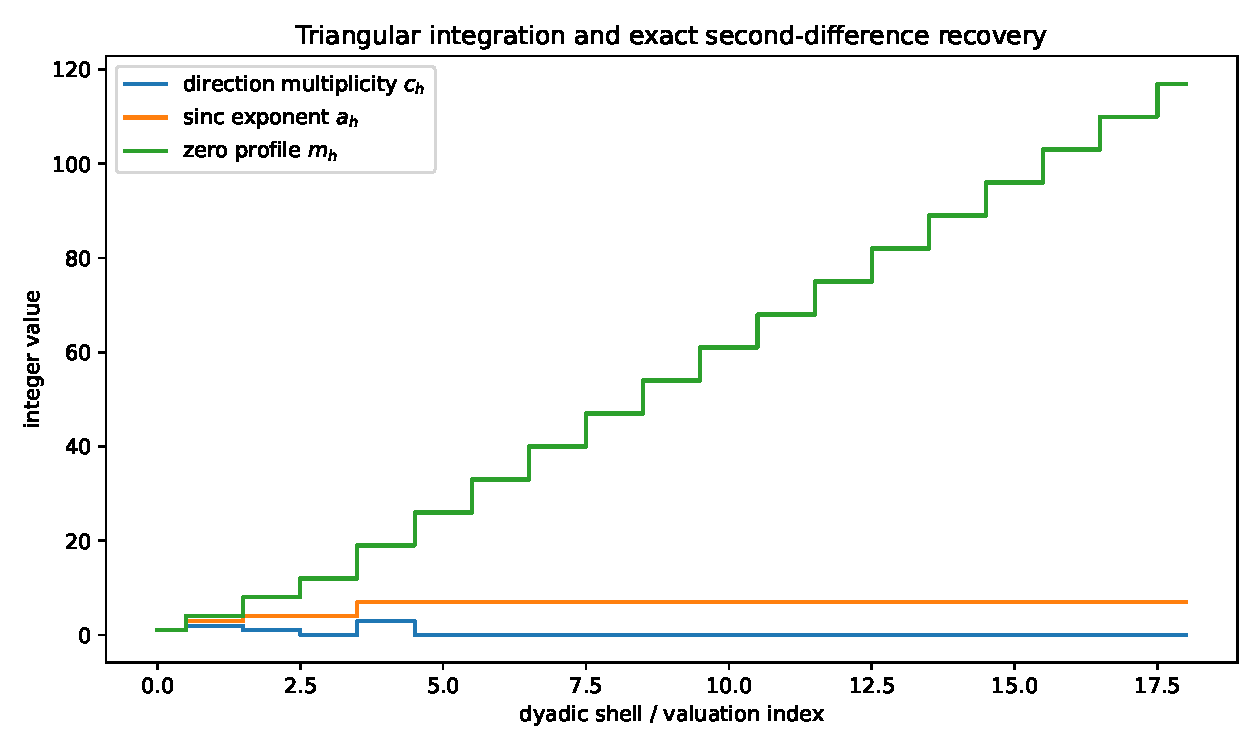
\includegraphics[width=0.92\textwidth]{figures/profile_inversion.pdf}
\caption{\Evidence\ A direction profile is integrated once to the sinc
exponents and twice to the integer-zero multiplicities.  The second difference
recovers the original profile exactly.}
\label{fig:profile-inversion}
\end{figure}

\subsection{Digital signs and Prouhet cancellation}

For four profiles, the sign computed from binary digits was compared with the
parity of all crossed sinc zeros for every $0\le N<1024$; all values agreed.
The script then checked 28 finite blocks.  In each block all power sums below
the order $d_M(c)$ vanished exactly.  For the classical profile, the first
nonzero sums at block sizes $8,16,32$ are respectively
$-48,1536,-122880$, in agreement with the exact Thue--Morse product.

\begin{figure}[H]
\centering
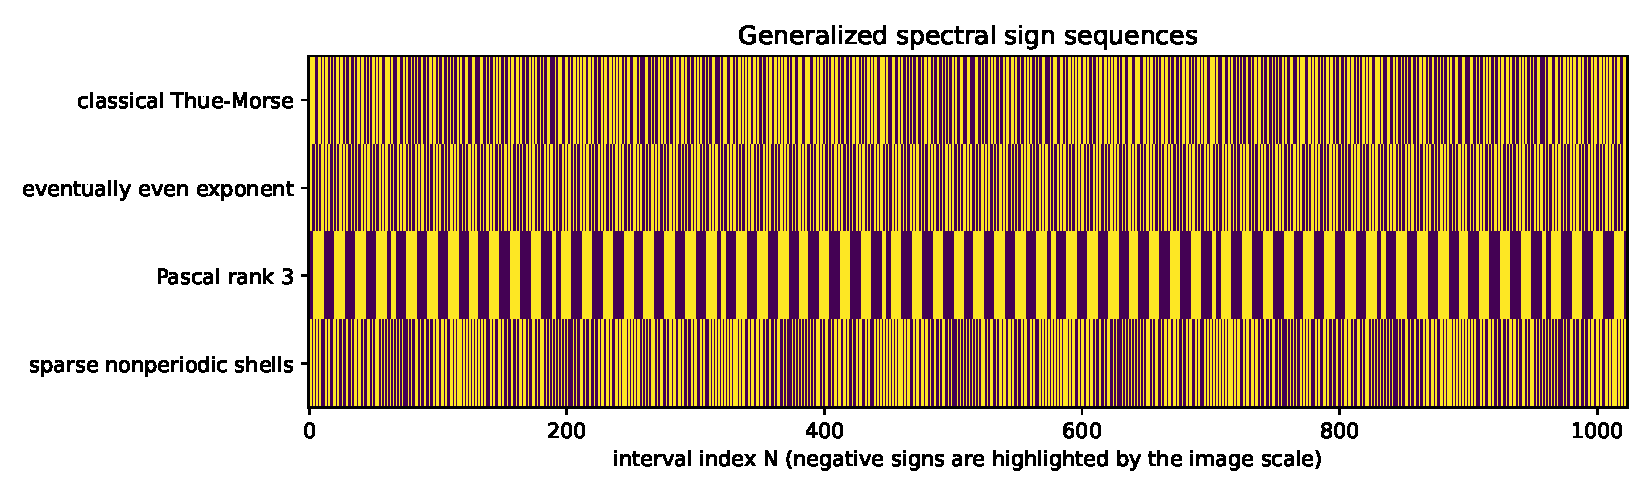
\includegraphics[width=0.98\textwidth]{figures/digital_signs.pdf}
\caption{\Evidence\ Prefixes of four generalized spectral sign sequences.
The third row is a Pascal mask; the fourth comes from sparse power-of-two
shells and is provably nonautomatic by \cref{thm:automaticity}.}
\label{fig:digital-signs}
\end{figure}

\subsection{Cumulant-ratio moments}

For the finite profile
\begin{equation}
 c=(2,1,3,1,2,2,1),
\end{equation}
the first ratios are
\begin{equation}
 R_1=\frac{10089}{4096},\quad
 R_2=\frac{34804257}{16777216},\quad
 R_3=\frac{138563297409}{68719476736}.
\end{equation}
All signed finite differences through order eight were nonnegative.  Exact
leading Hankel determinants through size six were strictly positive, as
predicted by the seven occupied dyadic atoms.

\begin{figure}[H]
\centering
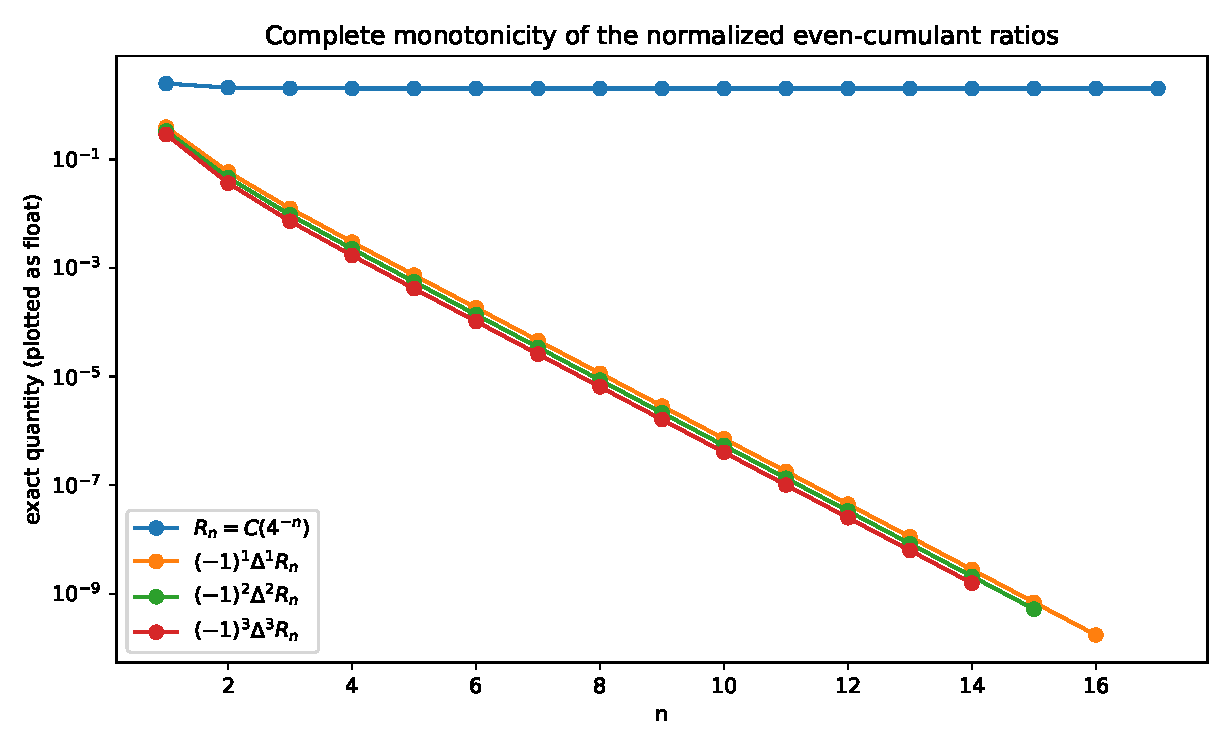
\includegraphics[width=0.92\textwidth]{figures/cumulant_ratio_moments.pdf}
\caption{\Evidence\ Complete monotonicity of the exact cumulant-ratio sequence.
The plotted floating values come from exact rational data.}
\label{fig:cumulant-ratios}
\end{figure}

\subsection{Zero zeta and Fourier envelope}

At $s=3.75$ for the profile $c=(1,2,0,3,1)$, the direct sum through
$N=500000$ agrees with \eqref{eq:zero-zeta} to an absolute error below
$3.8\times10^{-16}$.

For the exponent families $a_j=(j+1)^d$, $0\le d\le3$, the sharp ray
$x_H=2^H/3$ was evaluated through $H=500$.  The terminal ratios are:
\begin{center}
\begin{tabular}{rrrr}
\toprule
$d$ & $H$ & observed ratio & predicted constant\\
\midrule
0 & 500 & -0.7281923692 & -0.7213475204\\
1 & 500 & -0.3528989083 & -0.3468948302\\
2 & 500 & -0.2560241321 & -0.2502317256\\
3 & 500 & -0.2228908502 & -0.2166048418\\
\bottomrule
\end{tabular}

\end{center}
The slowly decaying $H^{-1}$ correction is visible, but all four curves move
toward their proved constants.

\begin{figure}[H]
\centering
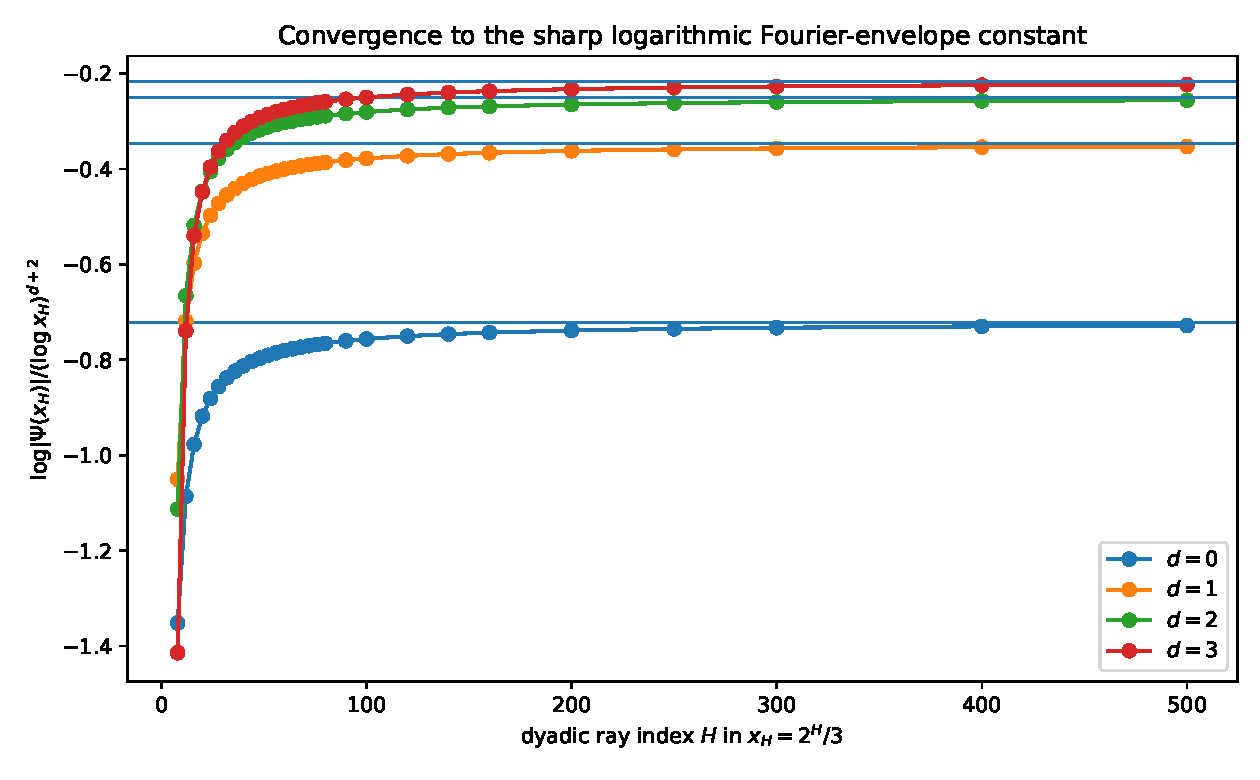
\includegraphics[width=0.92\textwidth]{figures/fourier_envelope.pdf}
\caption{\Evidence\ Convergence along the sharp rational dyadic ray.  The
horizontal lines are the constants in \eqref{eq:sharp-envelope}.}
\label{fig:fourier-envelope}
\end{figure}

\section{Conjectures and a frontier research program}
\label{sec:future}

\subsection{Spectral rigidity beyond the dyadic model}

\begin{conjecture}[\Conj\ Dyadic spectral rigidity]
\label{conj:spectral-rigidity}
Let
\[
 \Theta(t)=\prod_{\lambda\in\Lambda}\Phi(\lambda t)^{r_\lambda}
\]
be the characteristic function of a compactly supported projection of
independent up-laws, with positive coefficients $\lambda$ and integer
multiplicities $r_\lambda$.  Suppose every nonzero integer is a zero and its
multiplicity depends only on $\TwoAdicValuation(n)$.  After a common rescaling, every
$\lambda$ is a dyadic power and $\Theta=\Psi_c$ for a unique profile $c$.
\end{conjecture}

A possible proof should compare the smallest non-dyadic denominator in
$\Lambda$ with the exact integer zero set.  The obstruction is that different
scaled sinc zero lattices can overlap accidentally.  A divisor-theoretic
argument for entire functions of exponential type may isolate the dyadic
lattice.

\subsection{Stable $q$-tomography}

Exact recovery in \cref{prop:finite-reconstruction} is ill conditioned.  The
nodes $4^{-n}$ cluster at zero, so high shells contribute only beyond very
small scales.

\begin{problem}[Regularized profile recovery]
Develop error bounds for recovering a sparse or monotone integer profile from
noisy ratios $R_1,\ldots,R_N$.  Compare:
\begin{enumerate}[label=\textup{(\roman*)},leftmargin=*]
\item constrained geometric Vandermonde inversion;
\item Prony recovery of the dyadic Hausdorff measure $\mu_c$;
\item total-variation or $\ell^1$ regularization on the shell multiplicities;
\item modular reconstruction using the integrality of $c_h$.
\end{enumerate}
The objective is a theorem giving a recoverable shell depth as a function of
relative cumulant precision.
\end{problem}

\subsection{Tomography from several directions}

The present profile uses coefficients from the one-dimensional set
$\{2^{-h}\}$.  A product of several Fabius--Rvachev fields admits many linear
projections.

\begin{problem}[Finite-angle Fabius tomography]
Given a finite collection of dyadic projection directions, characterize when
the corresponding zero profiles determine the full multiset of coordinate
weights.  Seek analogues of discrete tomography uniqueness, switching
components, and compressed-sensing guarantees, with the integer zero divisor
as the measurement vector.
\end{problem}

\subsection{Base-$b$ and matrix-dilation profiles}

For an integer $b\ge2$, replace $2^{-h}$ by $b^{-h}$ and the rank-one atom by a
base-$b$ compactly supported refinable density.  The zero multiplicity then
samples $b$-adic valuations, while the sign sequence becomes a digit-weighted
$b$-kernel object.

\begin{conjecture}[\Conj\ Base-$b$ automaticity criterion]
Under a simple zero-lattice hypothesis, the spectral sign sequence of a
base-$b$ profile is $b$-automatic exactly when the shell-exponent residue word
modulo two is eventually periodic.  For odd $b$, the correct sign alphabet may
require more than two phases and should be expressed through roots of unity.
\end{conjecture}

A deeper extension replaces scalar dilation by an expanding integer matrix.
The direction generating function becomes multivariate, valuations are
replaced by divisibility along lattice orbits, and one expects a matrix Mahler
system rather than a scalar equation.

\subsection{Optimization of smoothness, support, and cubature precision}

At fixed support budget
$S_c=\sum_hc_h2^{-h}$, the precision at level $H$ is
\begin{equation}
 m_H=\sum_{h=0}^{H}c_h(H-h+1).
\end{equation}
Placing mass at coarse scales is expensive in support but contributes to many
future levels; fine-scale mass is cheap but arrives late.

\begin{problem}[Profile design]
Solve the integer optimization problems that maximize one or more of:
\begin{enumerate}[label=\textup{(\roman*)},leftmargin=*]
\item $m_H$ at a prescribed lattice level;
\item the asymptotic Fourier order $d+2$;
\item a weighted sum of exactness degrees over several levels;
\item conditioning of the positive cubature weights;
\end{enumerate}
subject to support, variance, or coordinate-count budgets.  Determine whether
Pascal profiles are extremal for any natural convex criterion.
\end{problem}

\subsection{Lambert phase tomography}

Conjecture \ref{conj:Lambert-profile} predicts that the singular jet of
$C(q)$ at $q=1$ controls the endpoint polynomial, while the dyadic complex
poles control periodic corrections.  A practical program is:
\begin{enumerate}[leftmargin=*]
\item derive the Mellin transform of \eqref{eq:Laplace-profile-log};
\item express its poles directly through $C(2^{-s})$;
\item obtain the large-$s$ Laplace exponent by residue summation;
\item solve the saddle equation in the coordinate
      \eqref{eq:profile-Lambert-coordinate};
\item transfer the result to the inverse-Fabius deficit sum
      \eqref{eq:deficit-inverse}.
\end{enumerate}
This would unify the rank-one and Pascal endpoint theories without assuming a
binomial exponent sequence.

\subsection{Arithmetic and exact-value questions}

Finite profiles have rational cumulants and moments, but pointwise values of
$g_c$ at dyadic rationals involve convolutions of up-values and need not inherit
the simplest rank-one denominator formulas.

\begin{problem}[Dyadic arithmetic of profile densities]
For finite profiles, determine:
\begin{enumerate}[label=\textup{(\roman*)},leftmargin=*]
\item whether every dyadic value of $g_c$ is rational;
\item exact denominator valuations in terms of $c$ and the point denominator;
\item $q$-binomial formulae for the convolution weights;
\item finite Thue--Morse representations compatible with
      \eqref{eq:sign-polynomial}.
\end{enumerate}
The Pascal factorization is a particularly structured test case.
\end{problem}

\section{Formalization roadmap}
\label{sec:formalization}

The main algebraic results are suitable for staged Lean formalization.

\subsection{Tier I: finite combinatorics}
\begin{enumerate}[leftmargin=*]
\item triangular sums $a_j=\sum_{h\le j}c_h$ and
      $m_v=\sum_{j\le v}a_j$;
\item second-difference inversion and eventual-affinity criterion;
\item finite sign product \eqref{eq:sign-polynomial};
\item exact Prouhet order at $z=1$;
\item Pascal hockey-stick factorization.
\end{enumerate}
These require no analysis beyond finite sums and polynomial multiplicities.

\subsection{Tier II: probability and generating functions}
\begin{enumerate}[leftmargin=*]
\item construction of $Y_c$ under the deterministic support bound;
\item characteristic-function rearrangement;
\item cumulant scaling and $C(4^{-n})$ sampling;
\item the atomic Hausdorff measure and Hankel positivity;
\item inverse-Fabius quantile transport.
\end{enumerate}

\subsection{Tier III: complex and Fourier analysis}
\begin{enumerate}[leftmargin=*]
\item exact zero orders of the infinite product;
\item Poisson summation for compactly supported $C^\infty$ functions;
\item uniform cubature sharpness;
\item the global Fourier upper bound and the rational-ray lower bound;
\item meromorphic continuation consequences of \eqref{eq:zero-zeta}.
\end{enumerate}

\subsection{Tier IV: conjectural endpoint analysis}
Formalization should follow, not precede, an analytic proof of the profile
Lambert transseries.  The likely reusable components are Mellin inversion,
residue bookkeeping on a vertical pole lattice, explicit estimates for
$W_{-1}$, and composition of periodic asymptotic scales.

\section{Conclusion}

A dyadic Radon profile turns many apparently separate parts of the
Fabius--Rvachev theory into different transforms of one nonnegative integer
sequence:
\begin{center}
\begin{tabularx}{0.92\textwidth}{@{}lX@{}}
\toprule
observable & transform of the profile \\
\midrule
sinc exponent & $a_j=\sum_{h\le j}c_h$ \\
integer-zero multiplicity & $m_v=\sum_{h\le v}c_h(v-h+1)$ \\
direction recovery & $c_v=\Delta^2m_v$ \\
zero zeta & $\zeta(s)C(2^{-s})/(1-2^{-s})$ \\
even cumulant ratio & $C(4^{-n})$ \\
Hausdorff measure & $\sum_hc_h4^{-h}\delta_{4^{-h}}$ \\
spectral sign & binary digit pairing with $a_j\bmod2$ \\
Prouhet order & number of odd exponents in a finite prefix \\
Fourier envelope & two cumulative integrations of the growth of $c_h$ \\
endpoint Laplace law & $\prod_hL_1(2^{-h}s)^{c_h}$ \\
\bottomrule
\end{tabularx}
\end{center}
The complete integer zero divisor determines the geometry; the even cumulants
provide a second, independent $q$-tomographic reconstruction; digital parity
produces generalized Thue--Morse sequences; and polynomial exponent growth
determines a sharp logarithmic Fourier constant.  The Pascal hierarchy is
revealed as an explicit arrangement of classical rank-one up-laws rather than
an unrelated family of atoms.

The next decisive step is an all-orders endpoint theorem for general profiles.
Such a theorem would make $C(q)$ the common source of the zero-zeta pole
lattice, the Fourier envelope, the inverse-Fabius deficit, and the nested
Lambert phase.  The finite-difference classification proved here isolates the
right parameter space for that program.

\appendix

\section{Proof supplements}
\label{app:proofs}

\subsection{Support and smoothness in the infinite product model}

The support argument in \cref{thm:profile-law} can be phrased entirely in
measure-theoretic terms.  Let
\[
 K_c=\prod_{h\ge0}\prod_{\ell=1}^{c_h}[-1,1]
\]
with the product topology.  The profile bound makes
$L_c(x)=\sum_{h,\ell}2^{-h}x_{h,\ell}$ a uniformly convergent series of
continuous functions, hence continuous.  For any $y\in[-S_c,S_c]$, the convex
set $K_c$ contains points mapped to $-S_c$ and $S_c$, and its continuous linear
image is convex, hence the whole interval.  Because the product up-measure has
support $K_c$, the push-forward support is $L_c(K_c)$.

For smoothness, if $h_0$ is occupied, remove one coordinate at that scale.  If
$\rho_{h_0}(x)=2^{h_0}\RvachevUp(2^{h_0}x)$, then
$g_c=\rho_{h_0}*\nu$ for a compactly supported probability measure $\nu$.
Every derivative is
$g_c^{(r)}=\rho_{h_0}^{(r)}*\nu$, proving global $C^\infty$ regularity and
compact support without differentiating an infinite product.

\subsection{Exact first nonzero Prouhet derivative}

Let $J_M=\{j<M:\alpha_j=1\}$.  Factoring at $z=1$ gives
\[
 E_{c,M}(z)
 =\prod_{j\in J_M}(1-z^{2^j})
  \prod_{j\notin J_M}(1+z^{2^j}).
\]
Therefore
\begin{equation}
 E_{c,M}^{(d_M)}(1)
 =d_M!\,(-1)^{d_M}
 2^{\sum_{j\in J_M}j}
 2^{M-d_M},
 \label{eq:first-Prouhet-derivative}
\end{equation}
which is nonzero.  This gives an exact falling-factorial moment at the first
surviving degree and can be converted to an ordinary-power moment with Stirling
numbers.

\subsection{A direct complete-monotonicity identity}

With $\Delta R_n=R_{n+1}-R_n$,
\begin{align*}
 (-1)^k\Delta^kR_{n+1}
 &=(-1)^k\sum_{j=0}^{k}(-1)^{k-j}\binom{k}{j}R_{n+j+1}\\
 &=\sum_hc_h4^{-(n+1)h}
   \sum_{j=0}^{k}(-1)^j\binom{k}{j}4^{-jh}\\
 &=\sum_hc_h4^{-(n+1)h}(1-4^{-h})^k.
\end{align*}
This is \eqref{eq:complete-monotonicity}.  Equality in a nontrivial Hankel
minor occurs precisely when the test polynomial vanishes on every occupied
atom of $\mu_c$.

\section{Selected exact data}
\label{app:data}

\subsection{Pascal direction profiles}

\begin{center}
\begin{tabular}{@{}crrrrrrrr@{}}
\toprule
$r\backslash h$ & 0&1&2&3&4&5&6&7 \\
\midrule
1&1&0&0&0&0&0&0&0\\
2&0&1&1&1&1&1&1&1\\
3&0&0&1&2&3&4&5&6\\
4&0&0&0&1&3&6&10&15\\
5&0&0&0&0&1&4&10&20\\
6&0&0&0&0&0&1&5&15\\
\bottomrule
\end{tabular}
\end{center}
Cumulative summation down each row produces
$\binom{h}{r-1}$, the exponent in \eqref{eq:Pascal-product}.

\subsection{First cumulant-ratio inequalities}

For every profile,
\begin{align*}
 R_2&\le R_1,\\
 R_3-2R_2+R_1&\ge0,\\
 R_1R_3-R_2^2&\ge0,\\
 \det\begin{pmatrix}R_1&R_2&R_3\\RealNumbers_2&R_3&R_4\\RealNumbers_3&R_4&R_5\end{pmatrix}&\ge0.
\end{align*}
These are necessary conditions for any proposed even-cumulant sequence to come
from a dyadic Radon profile.  They are not sufficient unless the representing
Hausdorff measure is additionally supported on the exact grid
$\{4^{-h}:h\ge0\}$ with masses divisible by $4^{-h}$ in the integer sense
specified by \eqref{eq:mu-c}.

\section{Corpus and reproducibility manifest}
\label{app:manifest}

\subsection{Source families screened}

\begin{longtable}{@{}p{0.31\textwidth}p{0.61\textwidth}@{}}
\toprule
Source family & Material screened for overlap \\
\midrule
\endfirsthead
\toprule Source family & Material screened for overlap \\
\midrule
\endhead
Primary exposition and glossary & normalization, random series, functional equations, exact values, moments, cumulants, inverse, notation \\
Lean walkthrough and theorem index & formalized Fabius/up interfaces, dyadic arithmetic, Bell/Appell and Fourier declarations \\
Canonical frontier synthesis & current theorem registers, conjectures, provenance, and absorbed historical drafts \\
Thue--Morse volumes & finite products, Prouhet cancellation, automatic and Mahler formulae, rarefaction, digital sums \\
Exponent and $q$-series volumes & $q$-Pochhammer, Gaussian binomials, geometric laws, inverse $q$-functions, cyclotomic limits \\
Spectra and arithmetic & zero multiplicities, determinants, heat traces, arithmetic rays, Pascal hierarchy, Fourier envelopes \\
Integration and transforms & Mellin/Laplace/Fourier/Cauchy/Stieltjes transforms, fractional calculus, quantile integrals \\
Inverse and sampling & inverse germs, Lambert--Bell expansions, self-sampling, comb quadrature, Appell reconstruction \\
Representation frontiers & Legendre/Jacobi/Chebyshev expansions, polynomial synthesis, multiresolution, operator models \\
Archived papers and revisions & classical Fabius/Rvachev sources, historical variants, frozen theorem formulations \\
Prior generated packages & Stein--Koopman, free/Boolean, hyperbolic-gamma, cyclotomic $q$, Pascal, and geometric-comb reports \\
\bottomrule
\end{longtable}

Exact and close-variant searches were made for: Radon projection, direction
profile, zero-profile inversion, second-difference multiplicity recovery,
cumulant tomography, dyadic Hausdorff measure, automaticity iff parity
periodicity, inverse-Fabius projection, and Pascal factorization into classical
up-laws.  No direct treatment of the theorem package above was found in the
audited snapshot.  This is a repository-relative absence statement, not a
global-priority certification.

\subsection{Archive contents}

\begin{center}
\begingroup\small
\begin{tabularx}{0.96\textwidth}{@{}p{0.50\textwidth}X@{}}
\toprule
Path & Purpose \\
\midrule
\path{dyadic_radon_profiles_fabius_rvachev.tex} & complete LaTeX manuscript \\
\path{dyadic_radon_profiles_fabius_rvachev.pdf} & compiled and visually inspected PDF \\
\path{numerical_experiments.py} & fully commented exact and high-precision experiment driver \\
\path{data/*.csv} & deterministic exact/numerical tables \\
\path{data/fourier_envelope_table.tex} & generated manuscript table \\
\path{figures/*.pdf} & vector figures used in the report \\
\path{figures/*.png} & raster inspection copies \\
\path{numerical_results.txt} & human-readable computation summary \\
\path{CORPUS_AUDIT.md} & current claim-oriented nonduplication audit \\
\path{corpus_inventory_2026-08-27.txt} & preserved recursive TeX path ledger \\
\path{README.txt} & build, reproduction, and file map \\
\path{requirements.txt} & Python dependencies \\
\path{SHA256SUMS.txt} & package integrity hashes \\
\bottomrule
\end{tabularx}
\end{center}
\endgroup

\begin{thebibliography}{99}

\bibitem{ProveItDocs}
V.~Reshetnikov,
\emph{ProveIt: Analysis/FabiusFunction documentation corpus},
GitHub repository,
\url{https://github.com/VladimirReshetnikov/ProveIt/tree/main/Analysis/FabiusFunction/docs},
accessed 30 August 2026.

\bibitem{Fabius1966}
J.~Fabius,
A probabilistic example of a nowhere analytic $C^\infty$-function,
\emph{Zeitschrift fuer Wahrscheinlichkeitstheorie und Verwandte Gebiete}
\textbf{5} (1966), 173--174.

\bibitem{Rvachev1990}
V.~A.~Rvachev,
Compactly supported solutions of functional-differential equations and their
applications,
\emph{Russian Mathematical Surveys} \textbf{45} (1990), no.~1, 87--120.

\bibitem{AriasUp}
J.~Arias de Reyna,
An infinitely differentiable function with compact support: definition and
properties,
\emph{Revista de la Real Academia de Ciencias Exactas, Fisicas y Naturales de
Madrid} \textbf{76} (1982), 21--38; English translation,
\url{https://arxiv.org/abs/1702.05442}.

\bibitem{AriasArithmetic}
J.~Arias de Reyna,
Arithmetic of the Fabius function,
\emph{INTEGERS} \textbf{18} (2018), Article A51;
\url{https://arxiv.org/abs/1702.06487}.

\bibitem{AlloucheShallit}
J.-P.~Allouche and J.~Shallit,
\emph{Automatic Sequences: Theory, Applications, Generalizations},
Cambridge University Press, 2003.

\bibitem{Comtet}
L.~Comtet,
\emph{Advanced Combinatorics},
D. Reidel, 1974.

\bibitem{CorlessLambert}
R.~M.~Corless, G.~H.~Gonnet, D.~E.~G.~Hare, D.~J.~Jeffrey, and D.~E.~Knuth,
On the Lambert $W$ function,
\emph{Advances in Computational Mathematics} \textbf{5} (1996), 329--359.

\bibitem{Helgason}
S.~Helgason,
\emph{The Radon Transform}, second edition,
Birkhauser, 1999.

\bibitem{ShohatTamarkin}
J.~A.~Shohat and J.~D.~Tamarkin,
\emph{The Problem of Moments},
American Mathematical Society, 1943.

\bibitem{Szego}
G.~Szego,
\emph{Orthogonal Polynomials}, fourth edition,
American Mathematical Society, 1975.

\bibitem{Titchmarsh}
E.~C.~Titchmarsh,
\emph{Introduction to the Theory of Fourier Integrals}, second edition,
Oxford University Press, 1948.

\end{thebibliography}

\end{document}
